\documentclass[11pt,letter]{article}
\usepackage[top=1.00in, bottom=1.0in, left=1.1in, right=1.1in]{geometry}
\renewcommand{\baselinestretch}{1}
\usepackage{graphicx}
\usepackage{natbib}
\usepackage{amsmath}
\usepackage{hyperref}
\usepackage{gensymb}
\usepackage{parskip}

\def\labelitemi{--}
\parindent=0pt

\begin{document}
\bibliographystyle{/Users/Lizzie/Documents/EndnoteRelated/Bibtex/styles/besjournals}
\renewcommand{\refname}{\CHead{}}

\setlength{\parindent}{0cm}
\setlength{\parskip}{5pt}

\title{Climate Hazards \\ Trying to organize results}
\author{Lizzie, Isabelle Chuine, Ben Cook, Victor van der Meersch}
\date{\today}
\maketitle
\tableofcontents
% A lot of this and the historical and mean warming results taken from 23 juin 2023 log notes to start with. 

\section{Historical trends}

\begin{itemize}
\item \emph{Fagus} is determined mainly by FruitIndex (related to frost damage). 
\item \emph{Pinus} survival dominates (due to carbon problems which comes from not enough chilling.) 
\item \emph{Quercus} is determined mainly MaturationIndex (does not mature in time) a little, but mostly it is fine. 
\end{itemize}

\begin{figure} 
 \begin{center}
\noindent 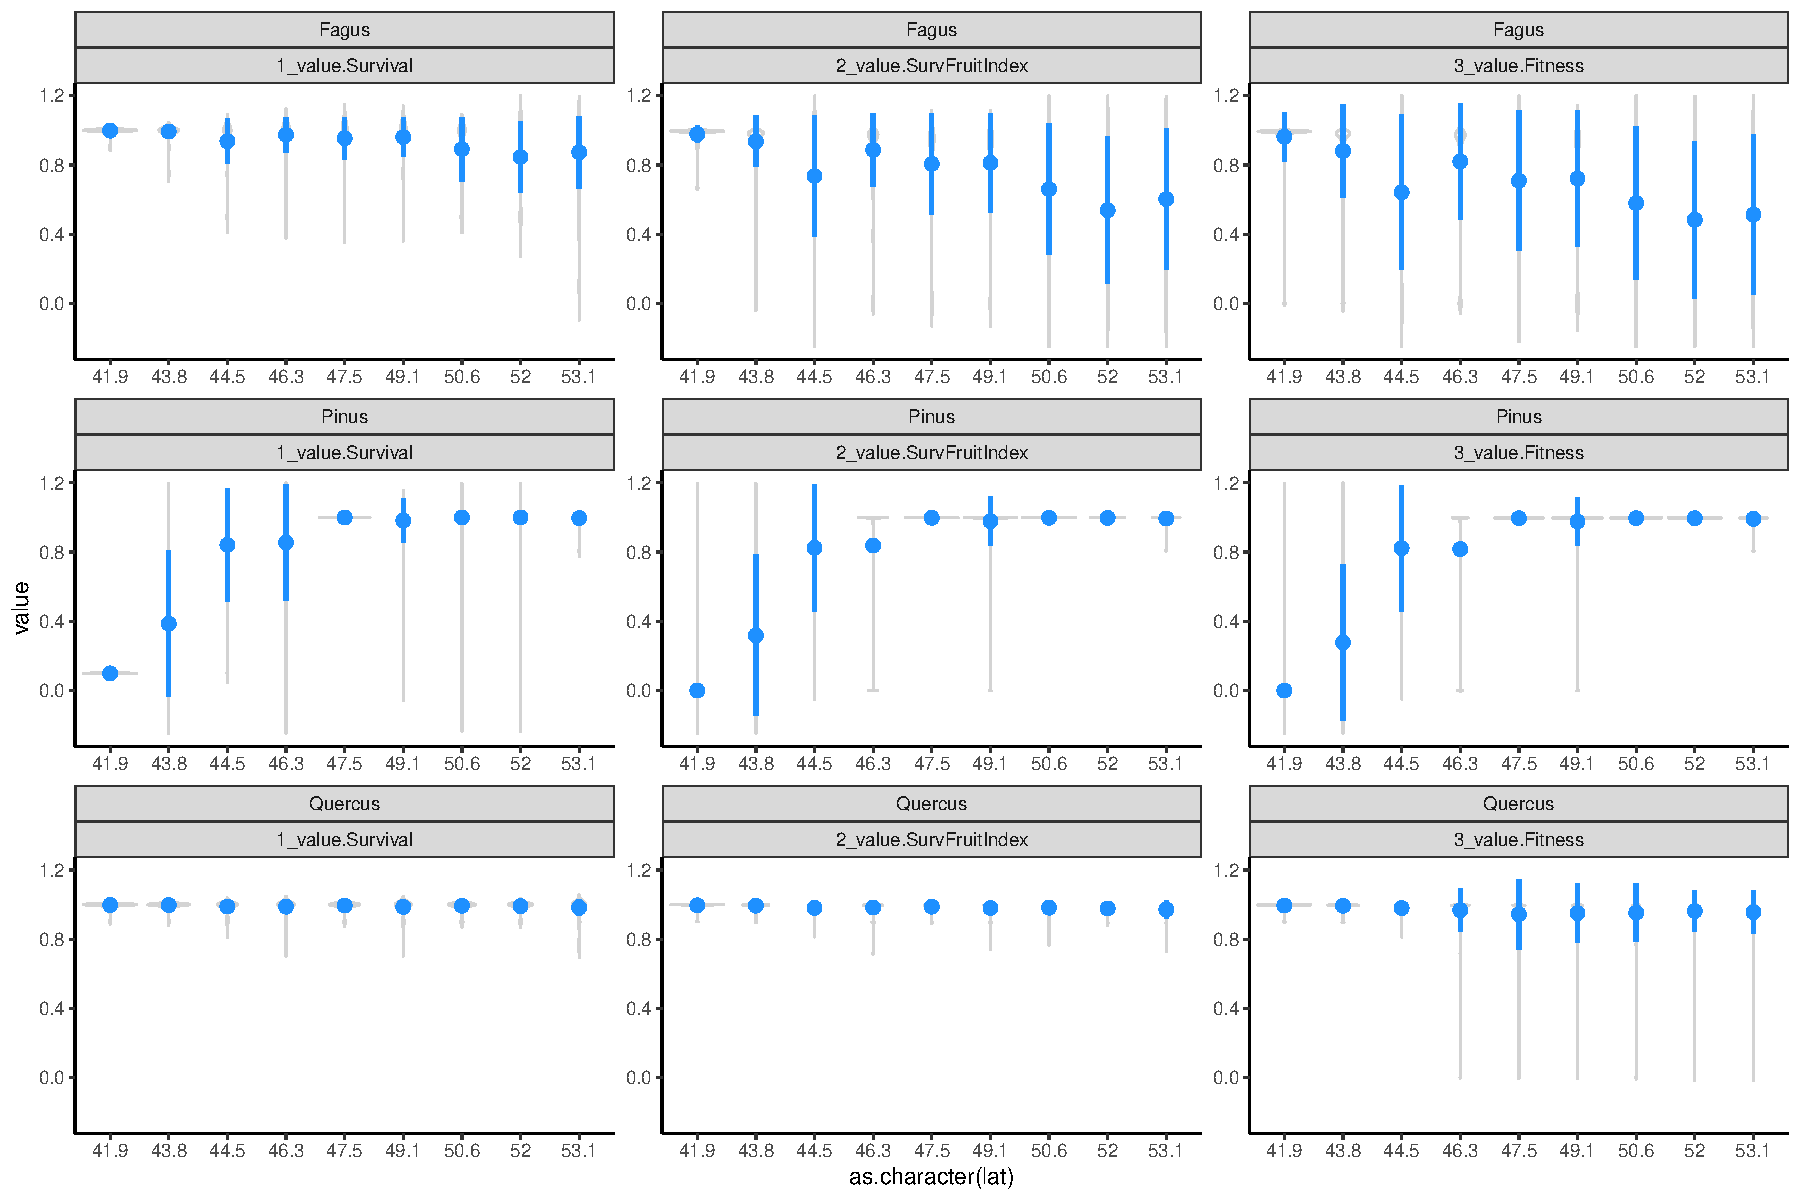
\includegraphics[width=1\textwidth]{..//analyses/graphs/phenofit/historical/fitnessBuildup.pdf}
  \caption{These results build through the multiplicative components of fitness (which are multiplied together): Survival (left), Survival$*$FruitIndex (middle) and Fitness, which is Survival$*$FruitIndex*MaturationIndex (right). Given high survival and little change between the middle and right panels we can see that \emph{Fagus} is determined mainly by FruitIndex (this makes sense as it is often affected by frost damage, having a low tolerance of low temperatures). We see next the for \emph{Pinus} survival dominates (often it does not meet the chill requirement for leafout and thus has no carbon and low CarbonSurvival so low total Survival) and finally, for \emph{Quercus} it's MaturationIndex (this makes sense as the fruits are quite large and can take a long time to mature---it doesn't always happen according to this model). }
  \label{fig:historicalfitnessl}
  \end{center}
\end{figure}

\newpage
\section{Overview of warming simulation results}

\subsection{\emph{Fagus} warming results}
Next the mean warming simulations. In understanding \emph{Fagus} results (Fig. \ref{fig:fagusmean3}) we discussed how we could see that at low latitudes (Fig. \ref{fig:fagusmean41}) that there was reduced CarbonSurvival (not enough cold means late dormancy) and thus FruitMaturationDate gets later. While at higher latitudes (Fig. \ref{fig:fagusmean53} ) there is an increase in the FruitIndex as FruitMaturation is higher. 


\begin{figure} 
 \begin{center}
\noindent 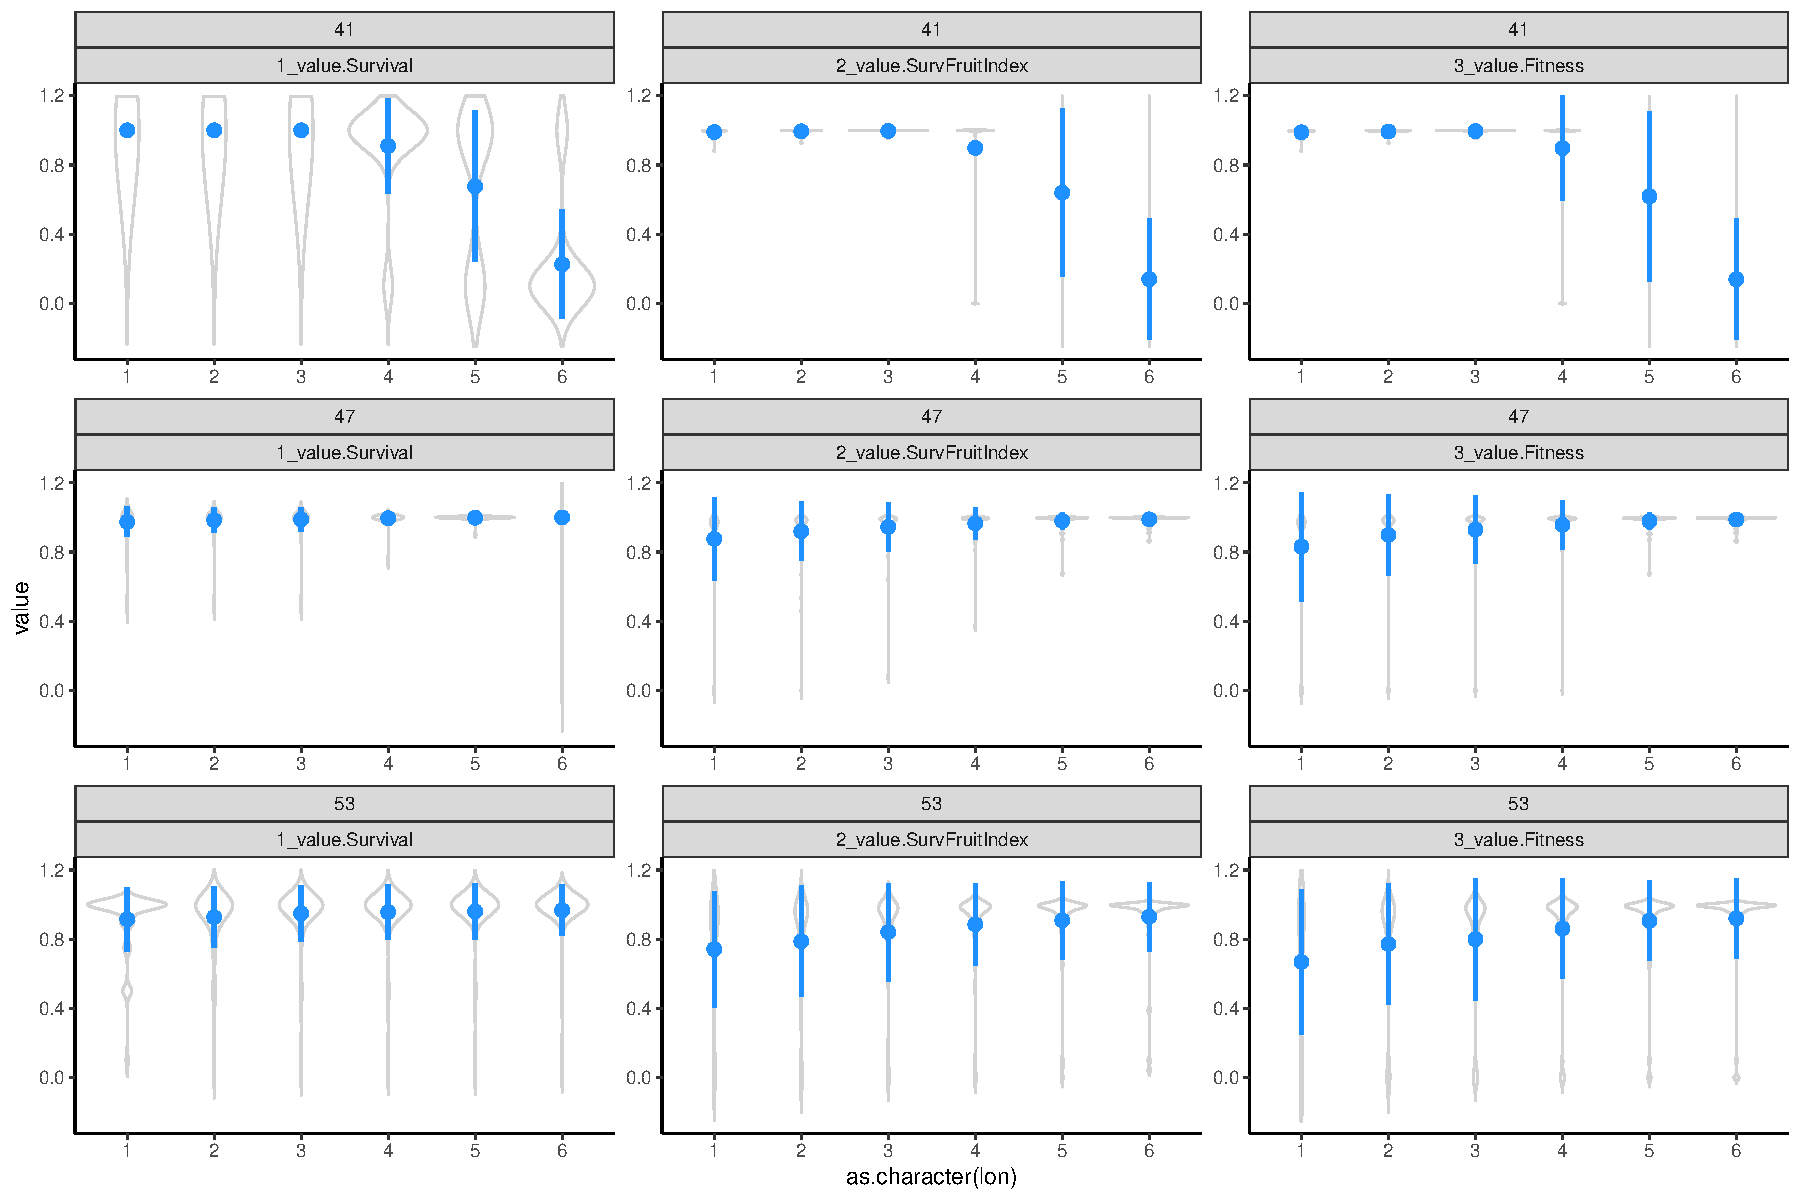
\includegraphics[width=1\textwidth]{..//analyses/graphs/phenofit/sims/metrics3/meansim_3metricsFS.pdf}
  \caption{\emph{Fagus} across 0 (1) to $+$5 (6) mean warming showing three latitudes. In June 2023, we discussed: at low latitudes (see next figure) that there was reduced CarbonSurvival (not enough cold means late dormancy) and thus FruitMaturationDate gets later. While at higher latitudes (see Fig. \ref{fig:fagusmean53}) there is an increase in the FruitIndex as FruitMaturation is higher.}
  \label{fig:fagusmean3}
  \end{center}
\end{figure}

\begin{figure} 
 \begin{center}
\noindent 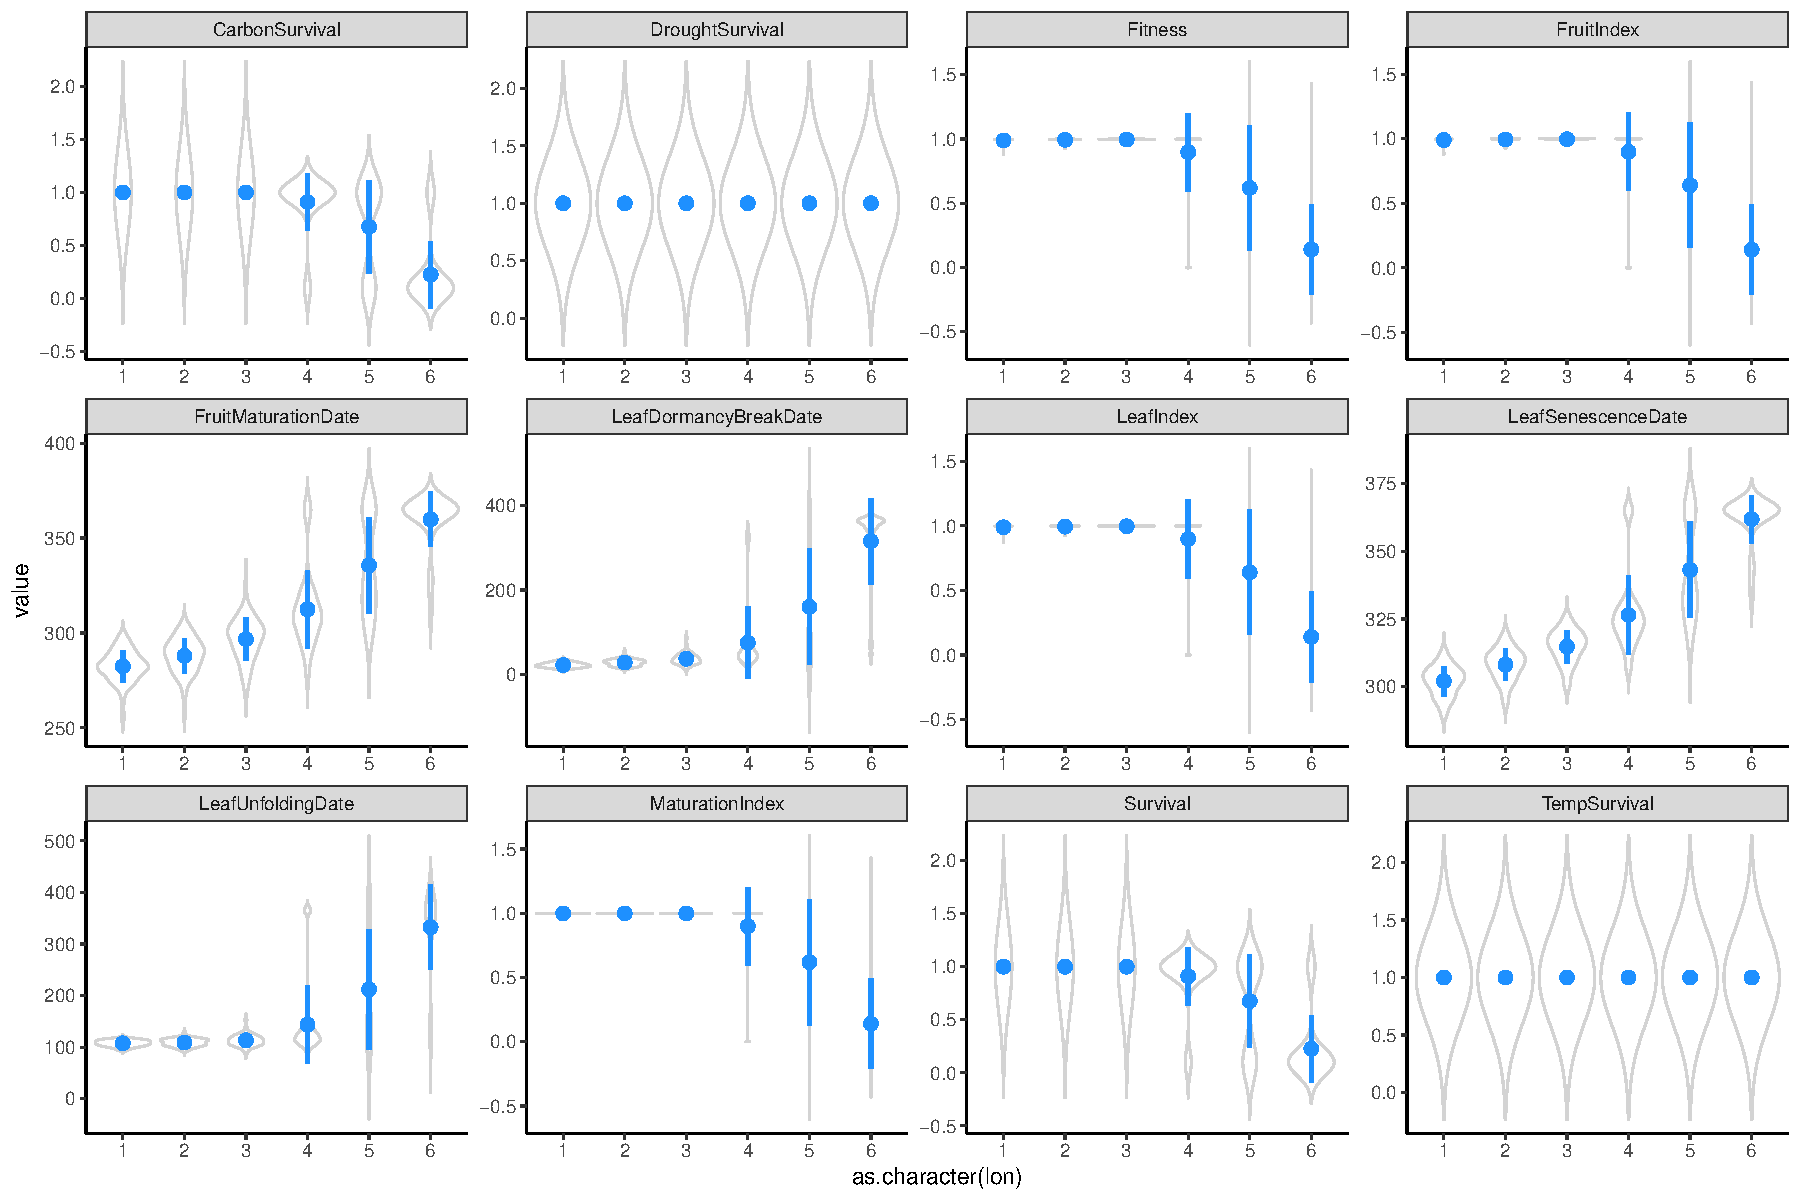
\includegraphics[width=1\textwidth]{..//analyses/graphs/phenofit/sims/meansim41_allmetricsFS.pdf}
  \caption{\emph{Fagus} across 0 (1) to $+$5 (6) mean warming across fitness components at 41\degree N latitude. Low fitness is driven by low carbonsurvival, which occurs because of late dormancy break date (because leafdormancybreakdate is variable that's the driver; if it were frost, we'd see more constant leafdormancybreakdate and variable in leafindex).}
  \label{fig:fagusmean41}
  \end{center}
\end{figure}

\begin{figure} 
 \begin{center}
\noindent 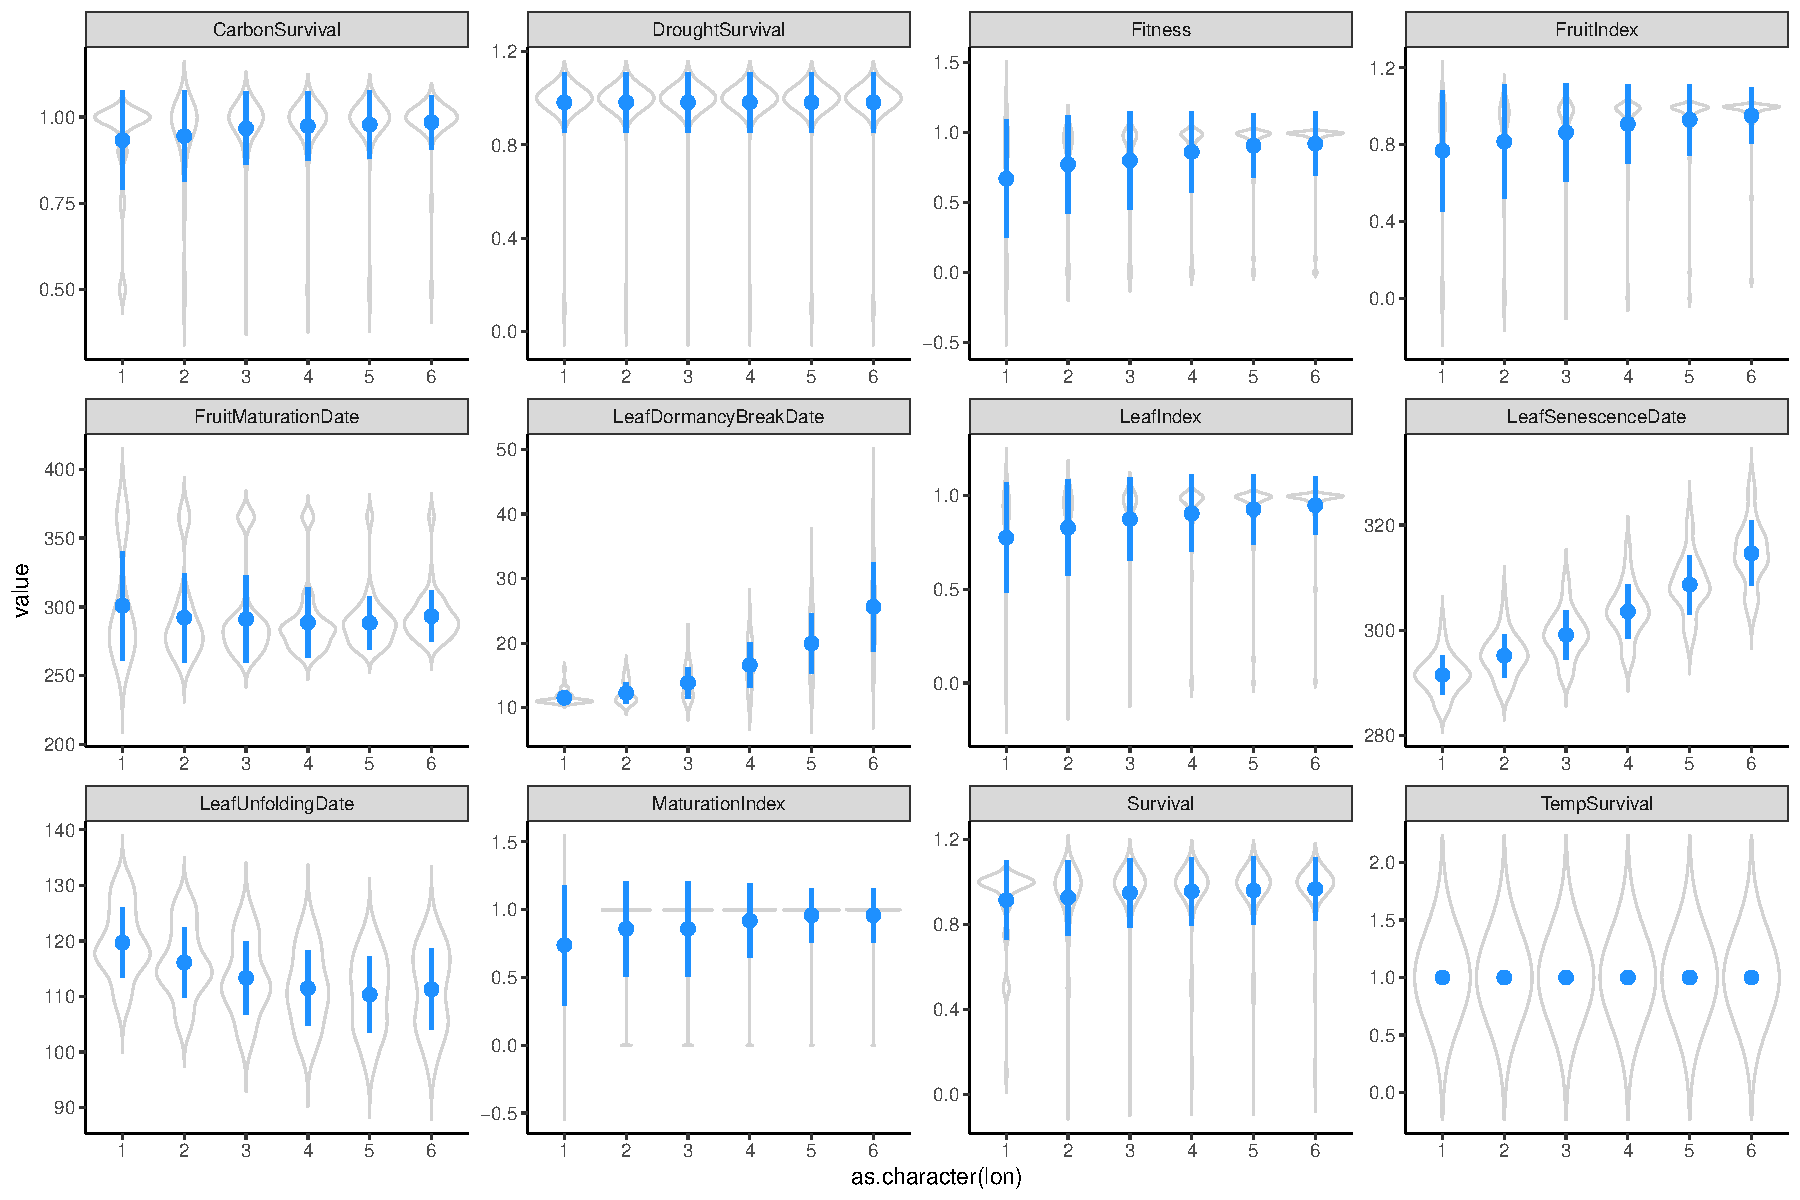
\includegraphics[width=1\textwidth]{..//analyses/graphs/phenofit/sims/meansim53_allmetricsFS.pdf}
  \caption{\emph{Fagus} across 0 (1) to $+$5 (6) mean warming across fitness components at 53\degree N latitude. Here's warming reduces frost and thus fruitindex goes up (less flowering damage probably) and survival goes up. MatIndex also goes up (likely due to a mix of leafindex going up and there is a direct effect of temperature on MatIndex). Note that the leafdormancybreakdate also gets a little later but leafunfolding does not because the warming is still enough for get earlier leafout (and there is a buffer where early dormancybreakdate does not matter because it's too cold leaf unfolding to start. }
  \label{fig:fagusmean53}
  \end{center}
\end{figure}

\clearpage
\subsection{For our mean results for  \emph{Pinus}}...
... it looks like carbon could be the issue again, which is close to 0 (minimum is 0.1 in PhenoFit for C survival) at low latitudes and declines with warming at the higher latitude. Check out dormancybreakdates which show that it must not get enough chilling. 

\begin{figure} 
 \begin{center}
\noindent 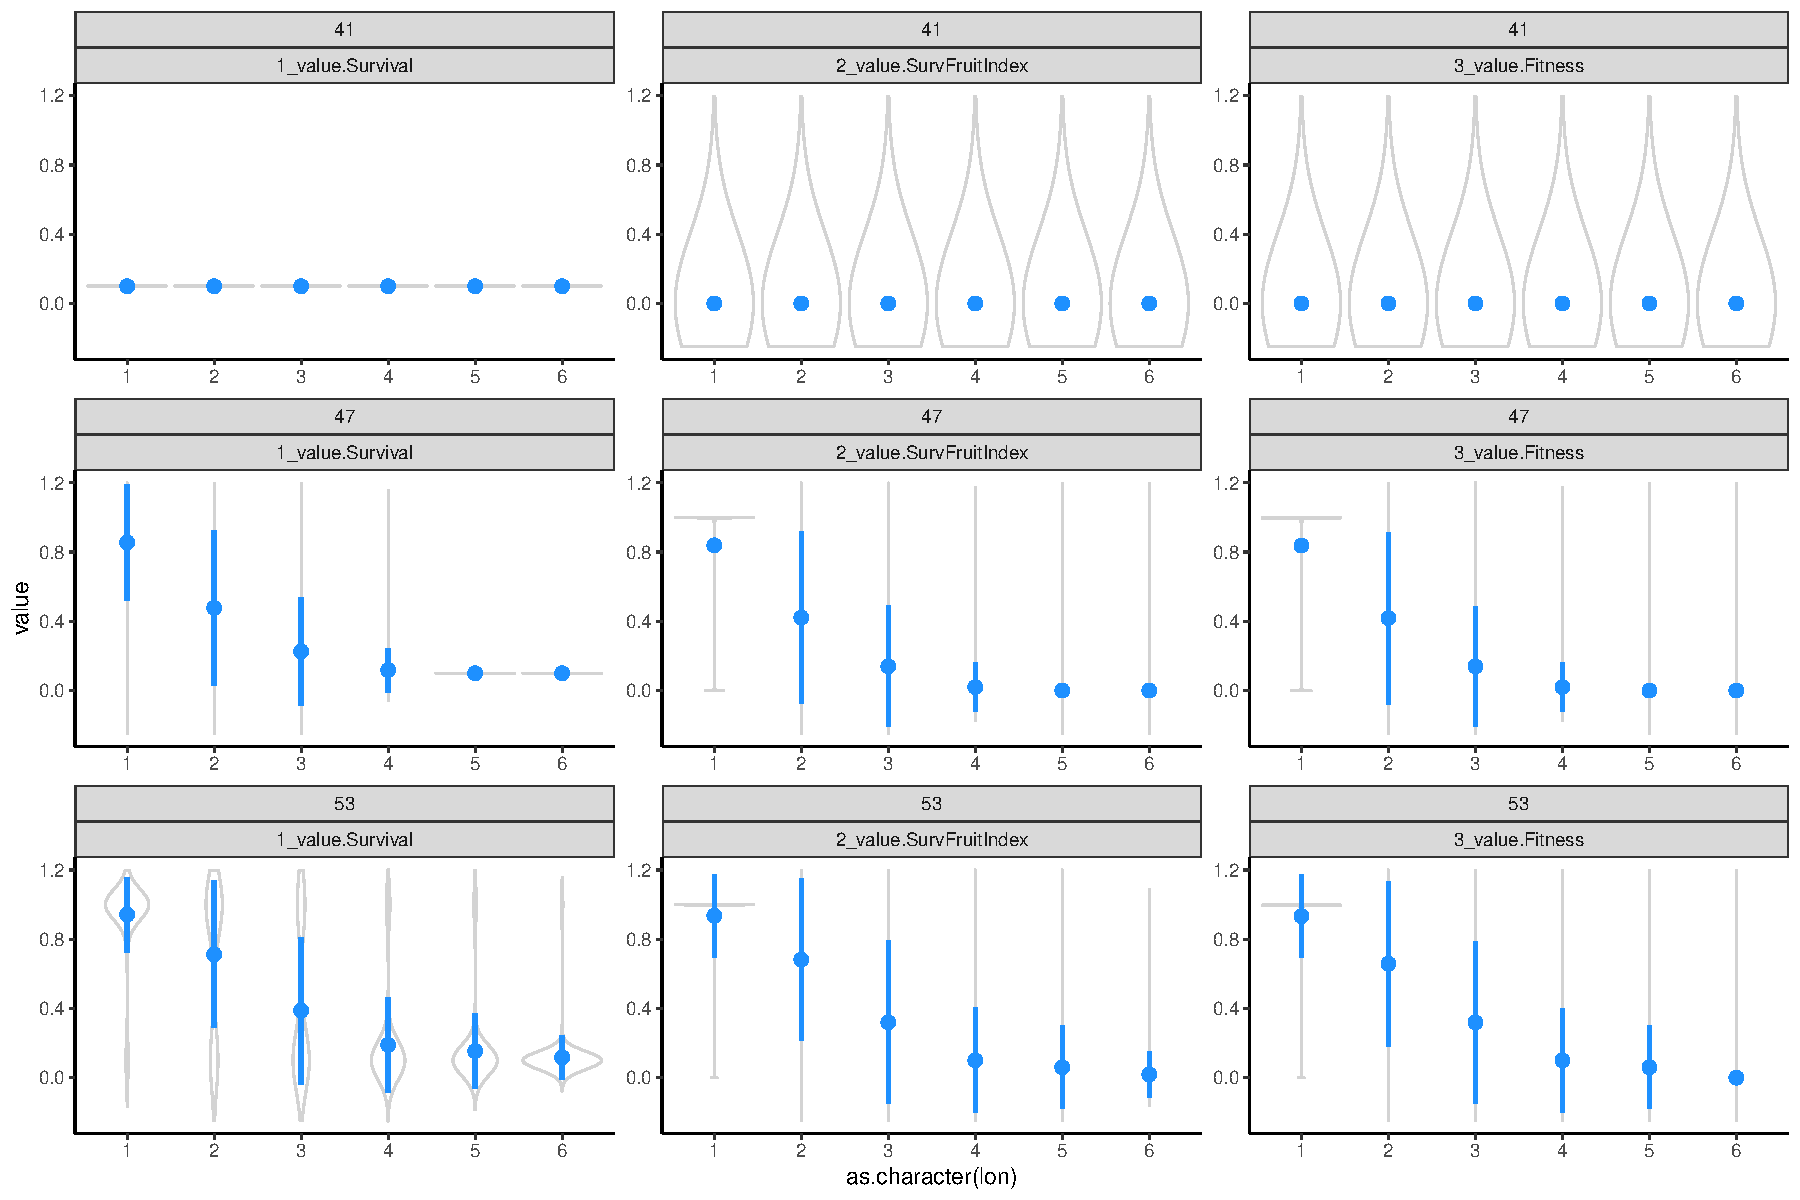
\includegraphics[width=1\textwidth]{..//analyses/graphs/phenofit/sims/metrics3/meansim_3metricsPS.pdf}
  \caption{\emph{Pinus} across 0 (1) to $+$5 (6) mean warming showing three latitudes. There is no survival at low latitudes, while at higher latitudes (see Fig. \ref{fig:pinusmean53}) warming leads to lower fitness due to low carbon survival (not enough chilling, so late dormancy break).}
  \label{fig:pinusmean3}
  \end{center}
\end{figure}

\begin{figure} 
 \begin{center}
\noindent 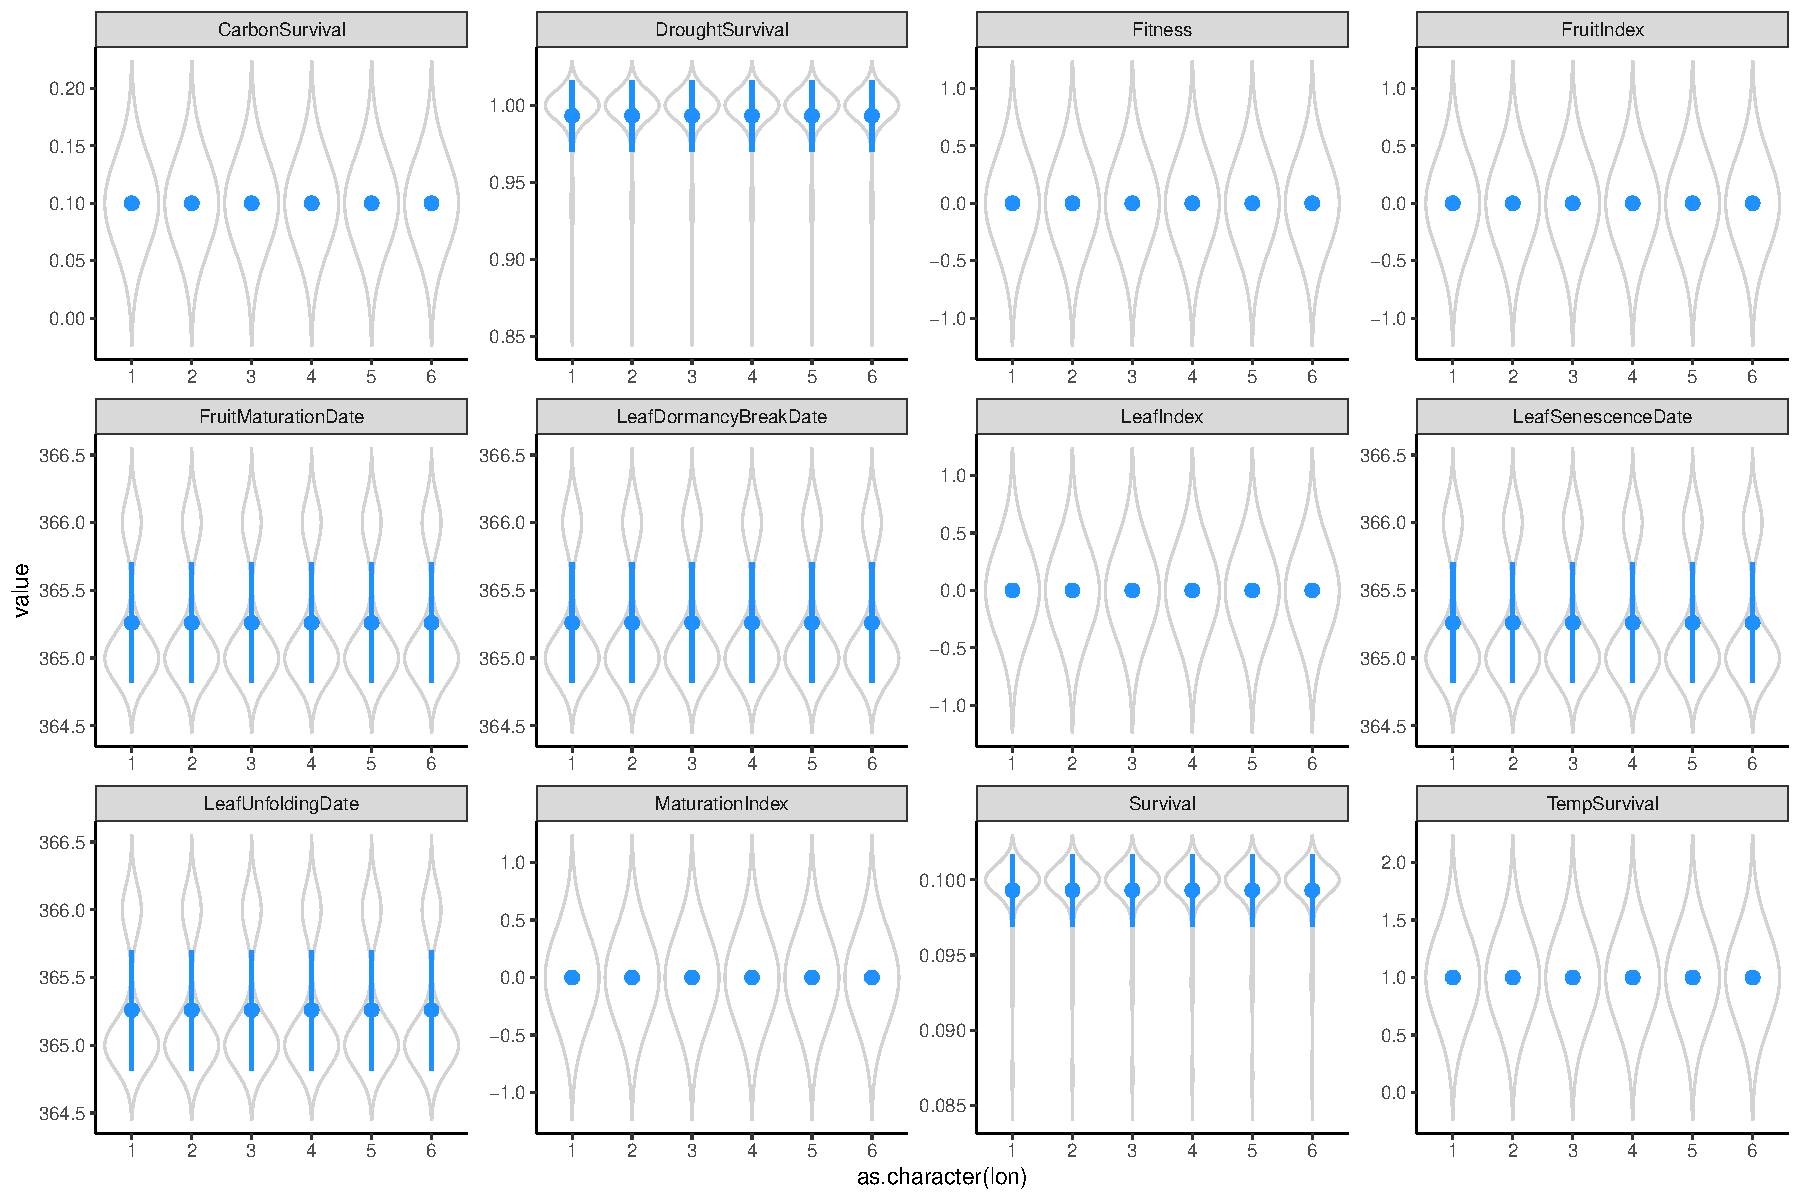
\includegraphics[width=1\textwidth]{..//analyses/graphs/phenofit/sims/meansim41_allmetricsPS.pdf}
  \caption{\emph{Pinus} across 0 (1) to $+$5 (6) mean warming across fitness components at 41\degree N latitude.}
  \label{fig:pinusmean41}
  \end{center}
\end{figure}

\begin{figure} 
 \begin{center}
\noindent 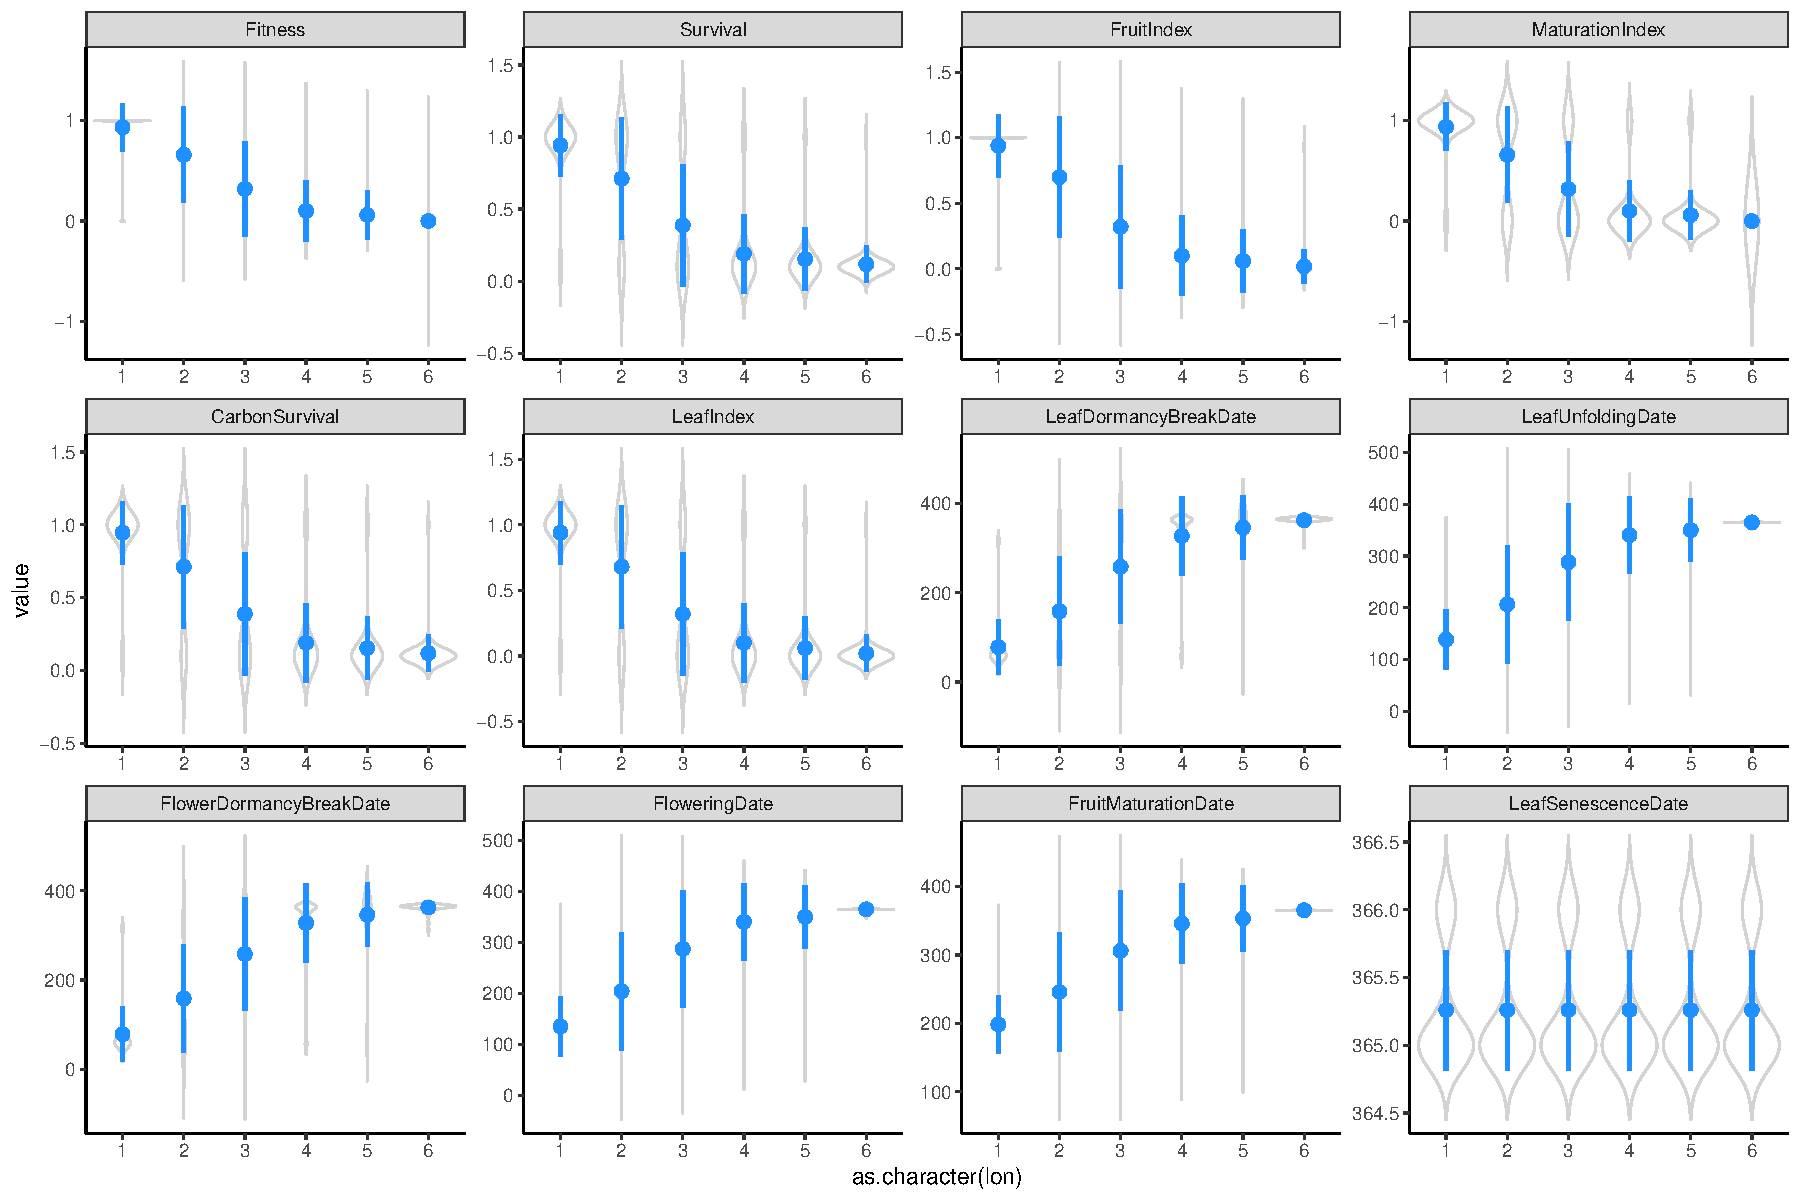
\includegraphics[width=1\textwidth]{..//analyses/graphs/phenofit/sims/meansim53_allmetricsPS.pdf}
  \caption{\emph{Pinus} across 0 (1) to $+$5 (6) mean warming across fitness components at 53\degree N latitude. See notes in caption of Fig. \ref{fig:pinusmean3}.}
  \label{fig:pinusmean53}
  \end{center}
\end{figure}

\clearpage

\subsection{For the mean results for \emph{Quercus} it is doing very well!}

\begin{figure} 
 \begin{center}
\noindent 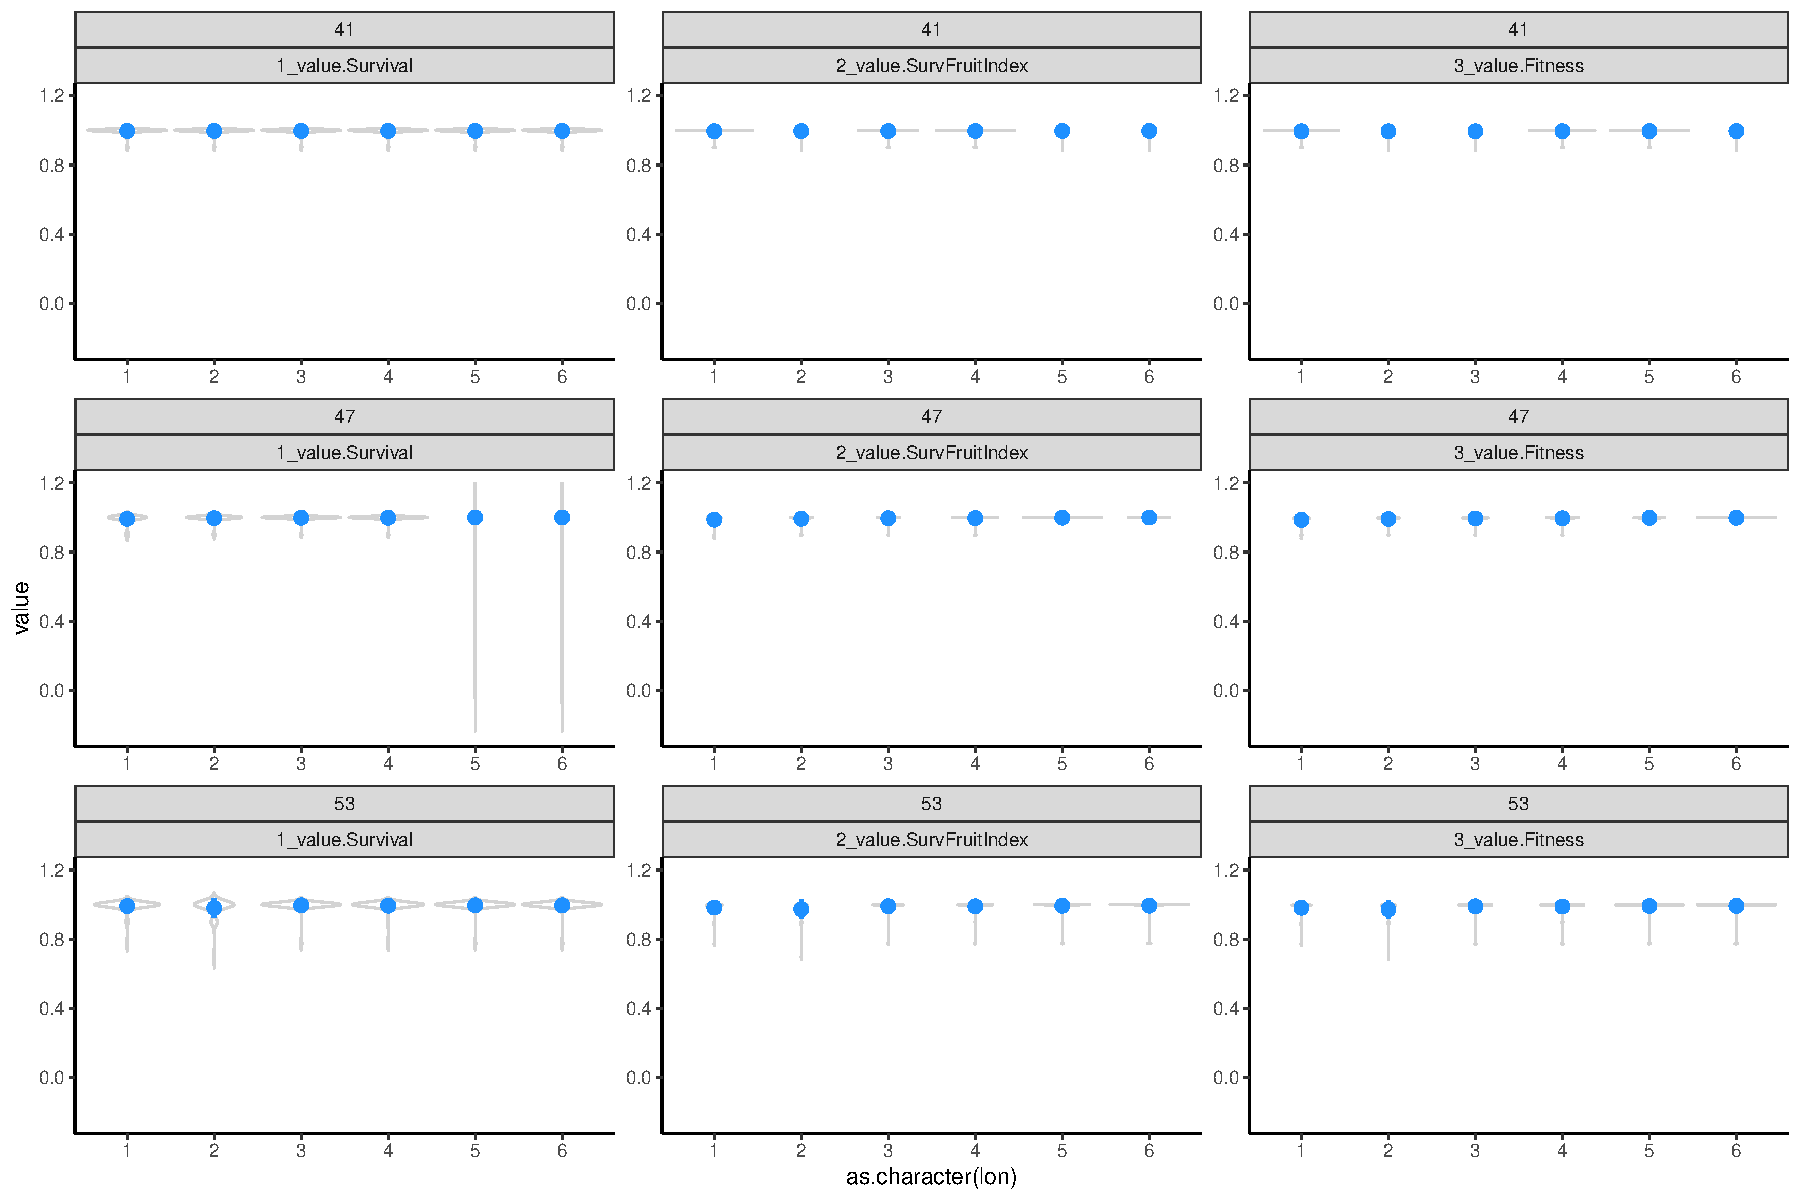
\includegraphics[width=1\textwidth]{..//analyses/graphs/phenofit/sims/metrics3/meansim_3metricsQR.pdf}
  \caption{\emph{Quercus} across 0 (1) to $+$5 (6) mean warming showing three latitudes.}
  \label{fig:quercusmean3}
  \end{center}
\end{figure}

\begin{figure} 
 \begin{center}
\noindent 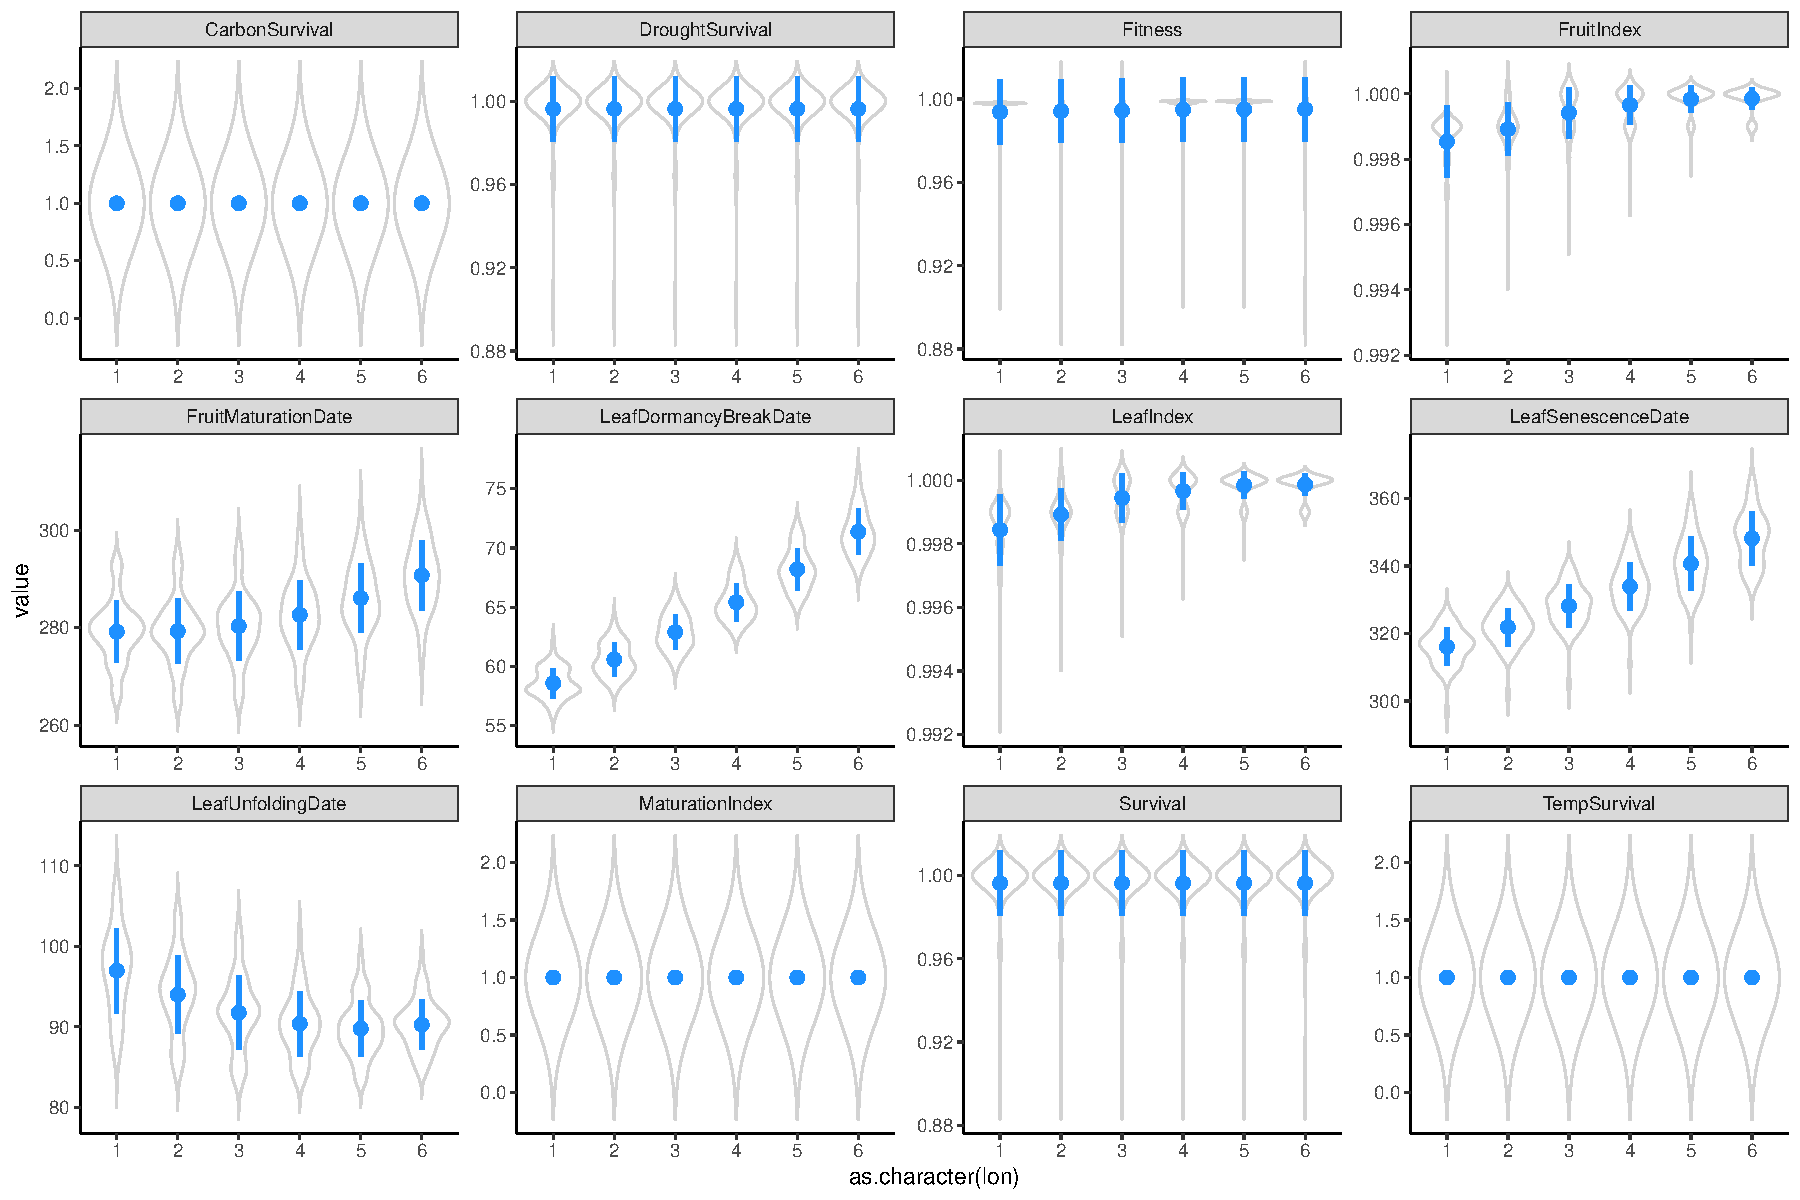
\includegraphics[width=1\textwidth]{..//analyses/graphs/phenofit/sims/meansim41_allmetricsQR.pdf}
  \caption{\emph{Quercus} across 0 (1) to $+$5 (6) mean warming across fitness components at 41\degree N latitude. }
  \label{fig:quercusmean41}
  \end{center}
\end{figure}

\begin{figure} 
 \begin{center}
\noindent 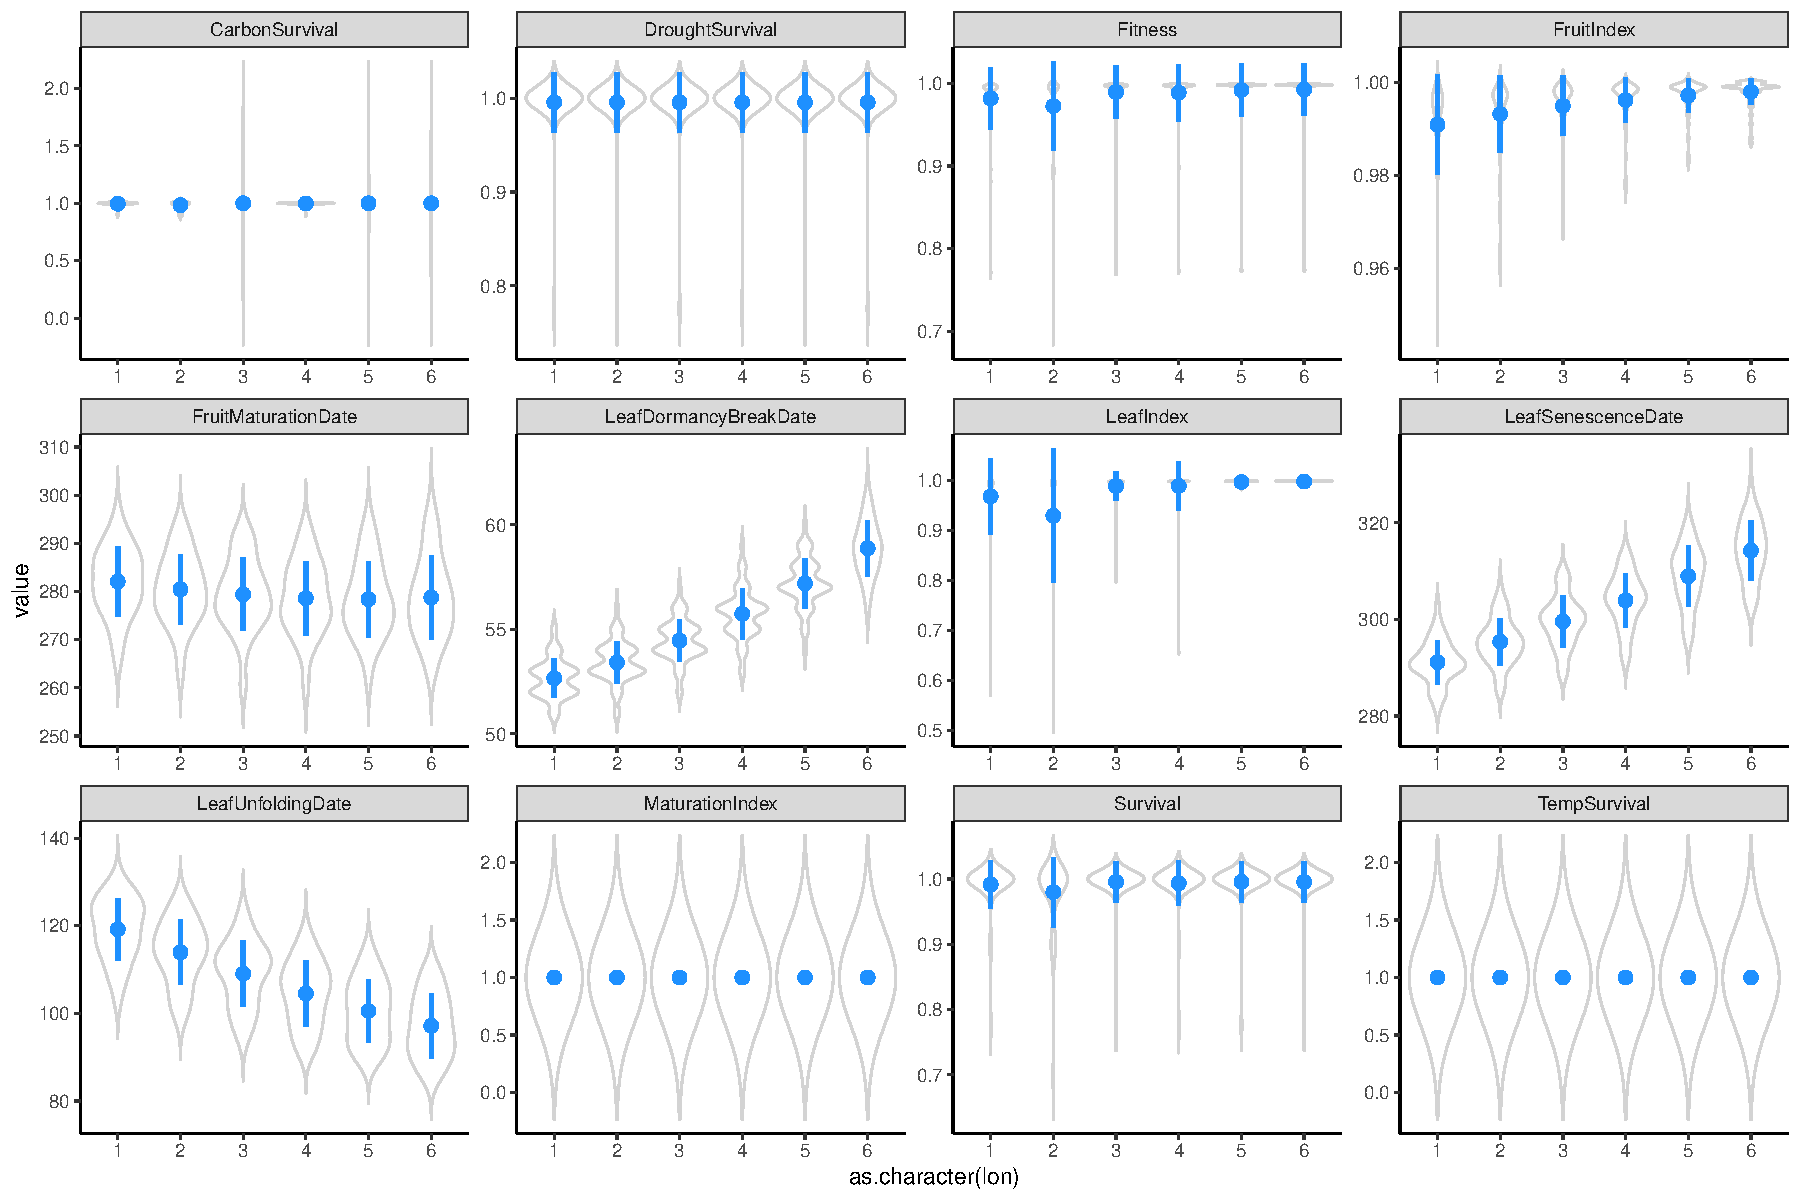
\includegraphics[width=1\textwidth]{..//analyses/graphs/phenofit/sims/meansim53_allmetricsQR.pdf}
  \caption{\emph{Quercus} across 0 (1) to $+$5 (6) mean warming across fitness components at 53\degree N latitude. }
  \label{fig:quercusmean53}
  \end{center}
\end{figure}

\newpage
\section{Overview of SD simulation results}

\begin{itemize}
\item \emph{Fagus} is determined mainly by a combo of damage to leaves and flowers, which increases with increasing variance. 
\item \emph{Pinus} survival dominates at low latitudes (no carbon survival and variance does not change this), but at highest latitude variance also leads to later leafout (low chill, later dormancy break) and thus lower leafindex (note that Pinus can sustain VERY low temperatures and is unlikely to have frost damage). 
\item \emph{Quercus} is not changing much but does see some frost losses at higher variance.
\end{itemize}


\begin{figure} 
 \begin{center}
\noindent 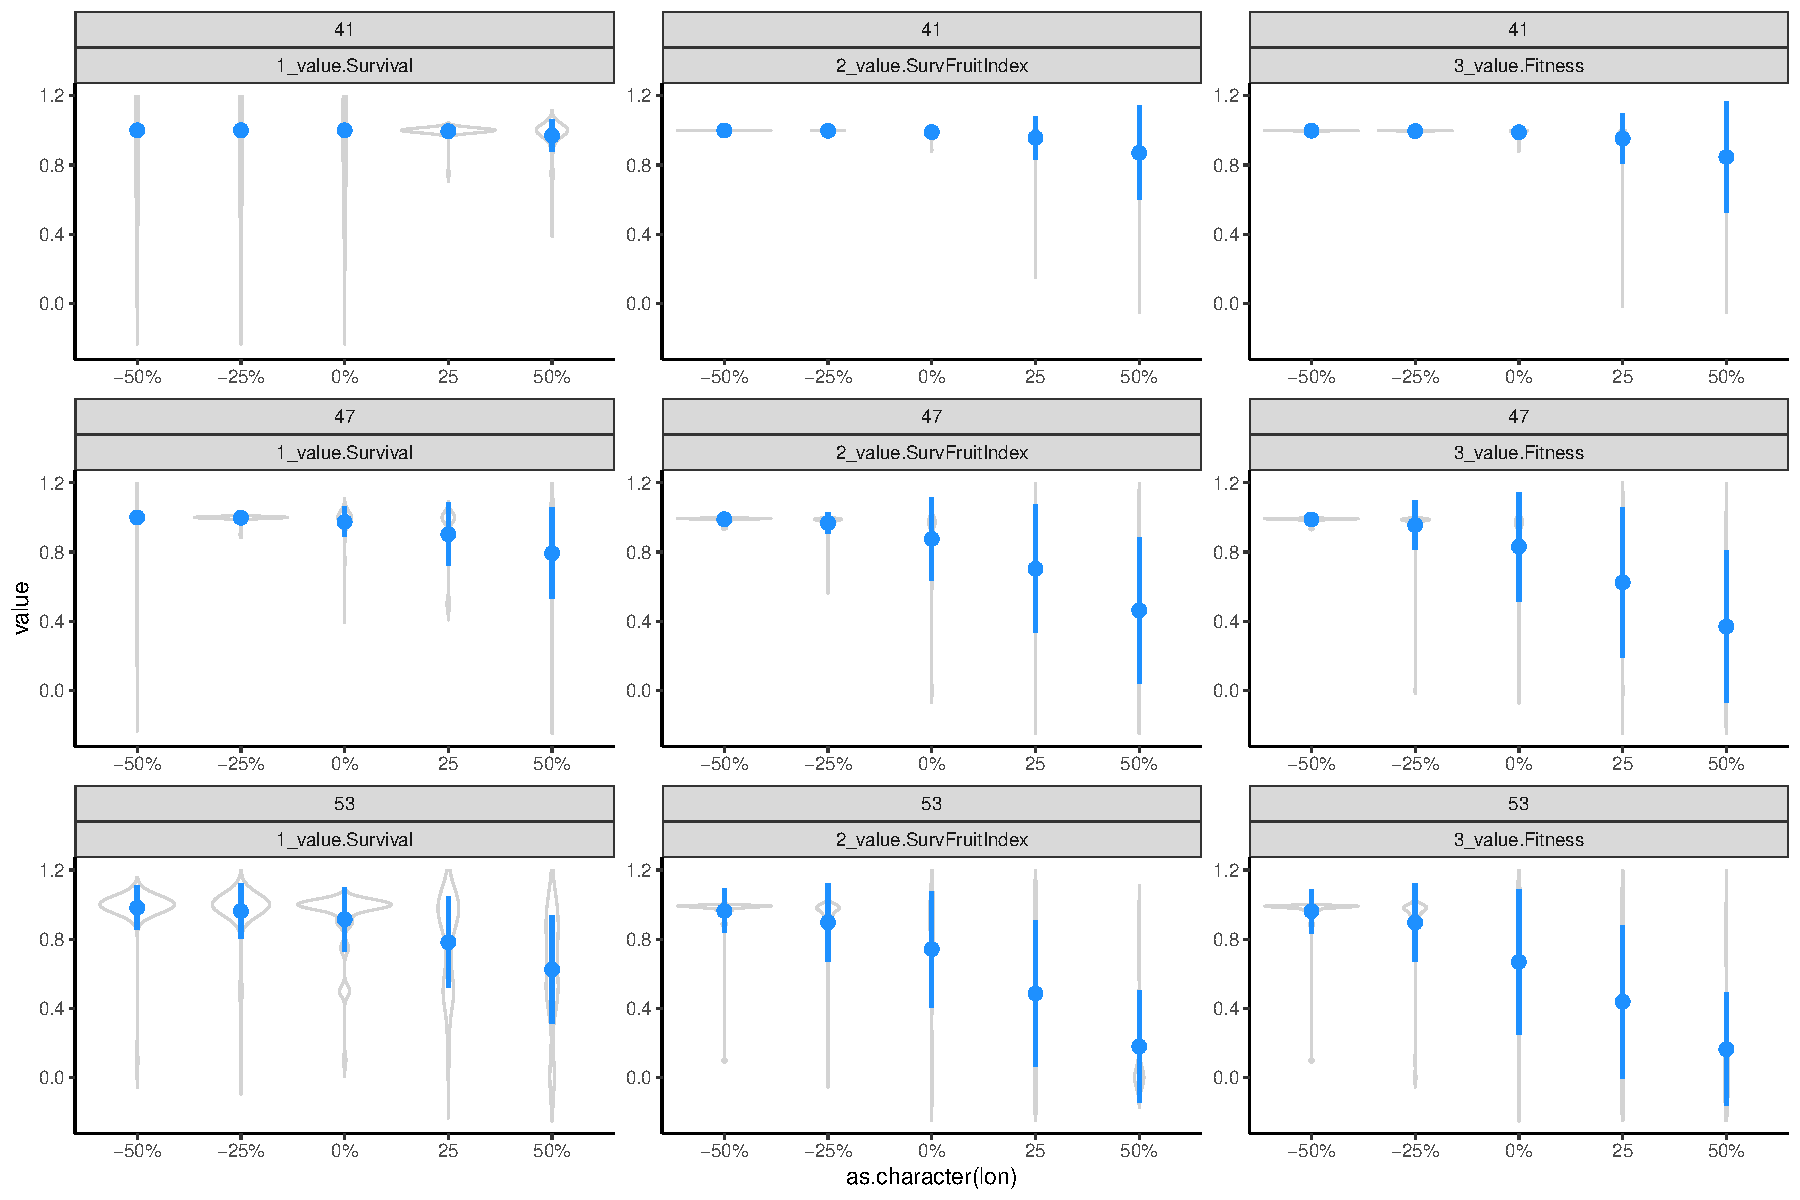
\includegraphics[width=1\textwidth]{..//analyses/graphs/phenofit/sims/metrics3/sdsim_3metricsFS.pdf}
  \caption{\emph{Fagus} across changing variance showing three latitudes. ...}
  \label{fig:fagussd3}sd
  \end{center}
\end{figure}

\begin{figure} 
 \begin{center}
\noindent 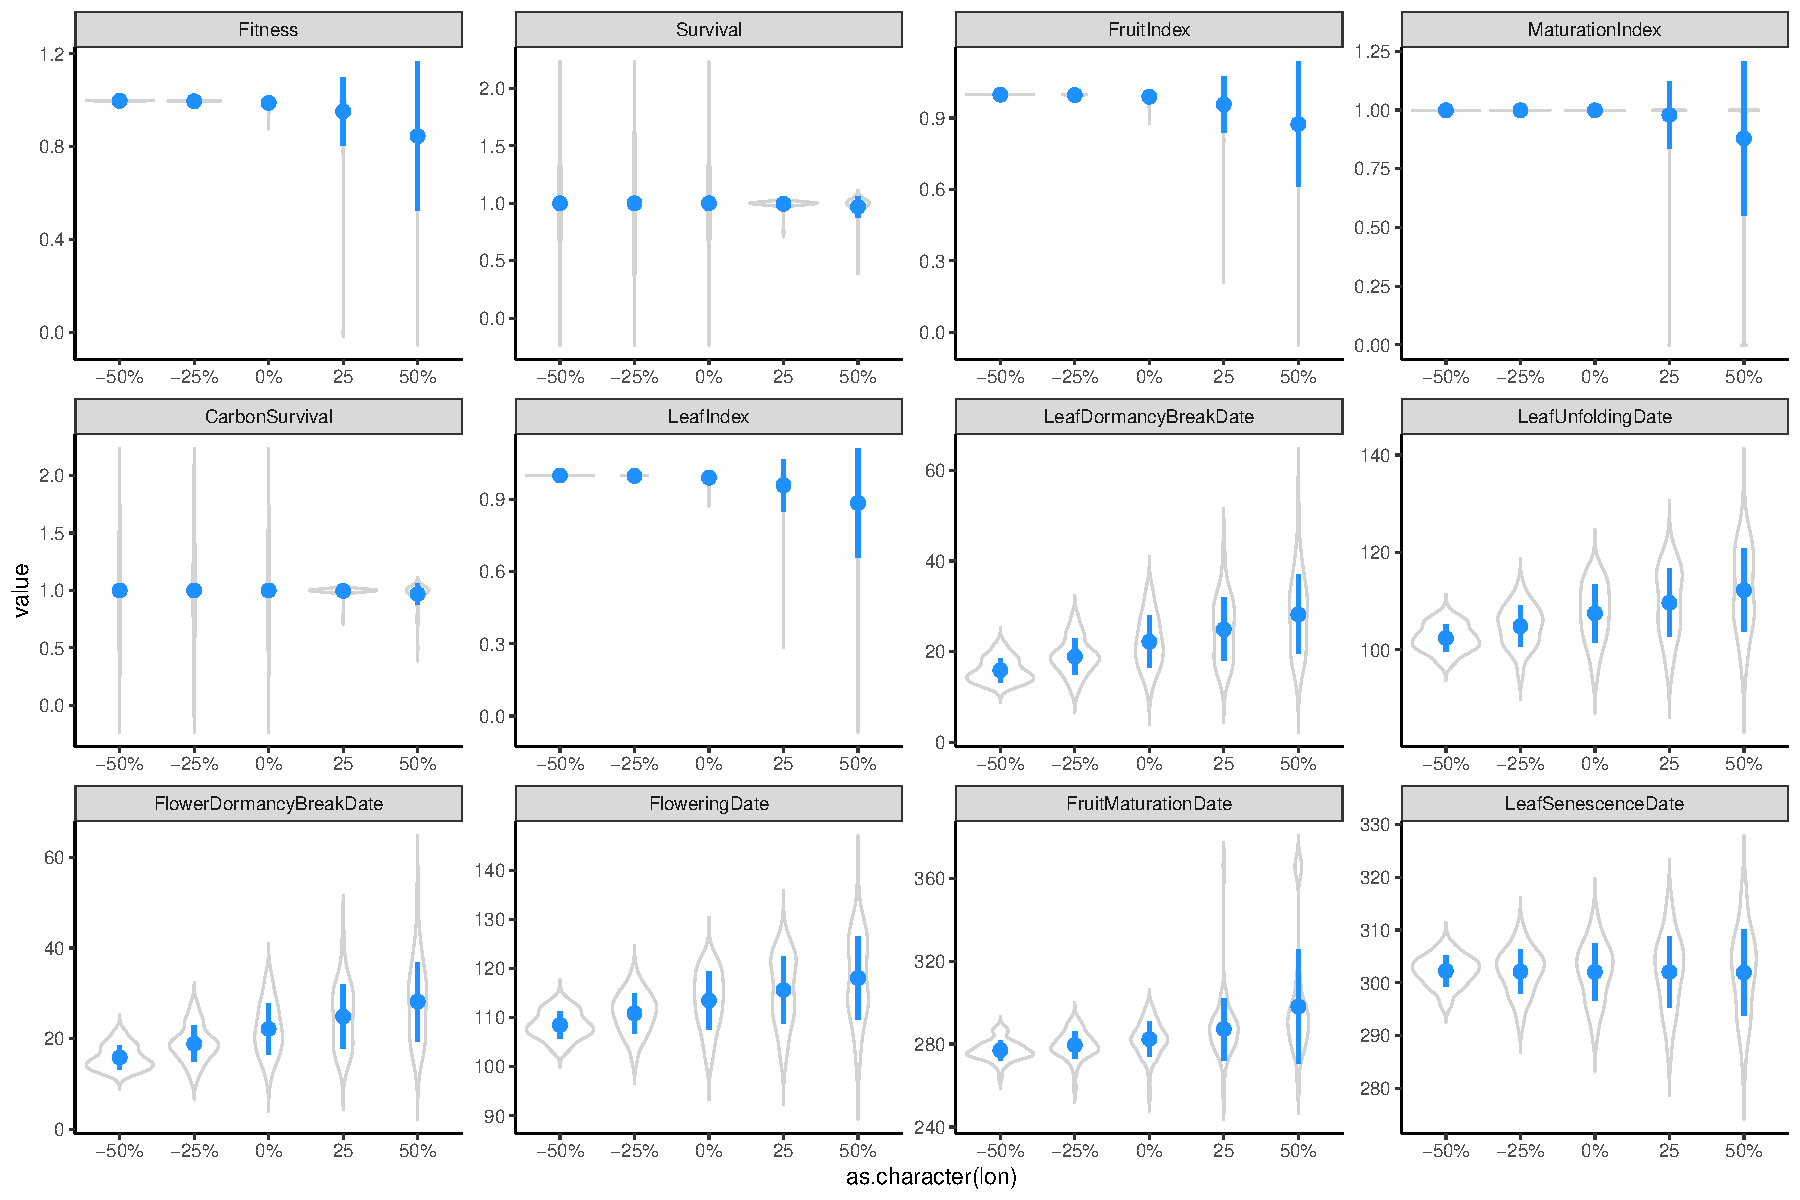
\includegraphics[width=1\textwidth]{..//analyses/graphs/phenofit/sims/sdsim41_allmetricsFS.pdf}
  \caption{\emph{Fagus} across changing variance across fitness components at 41 latitude. Low fitness is driven by low carbonsurvival, which occurs because of late dormancy break date (because leafdormancybreakdate is variable that's the driver; if it were frost, we'd see more constant leafdormancybreakdate and variable in leafindex).}
  \label{fig:fagussd41}
  \end{center}
\end{figure}

\begin{figure} 
 \begin{center}
\noindent 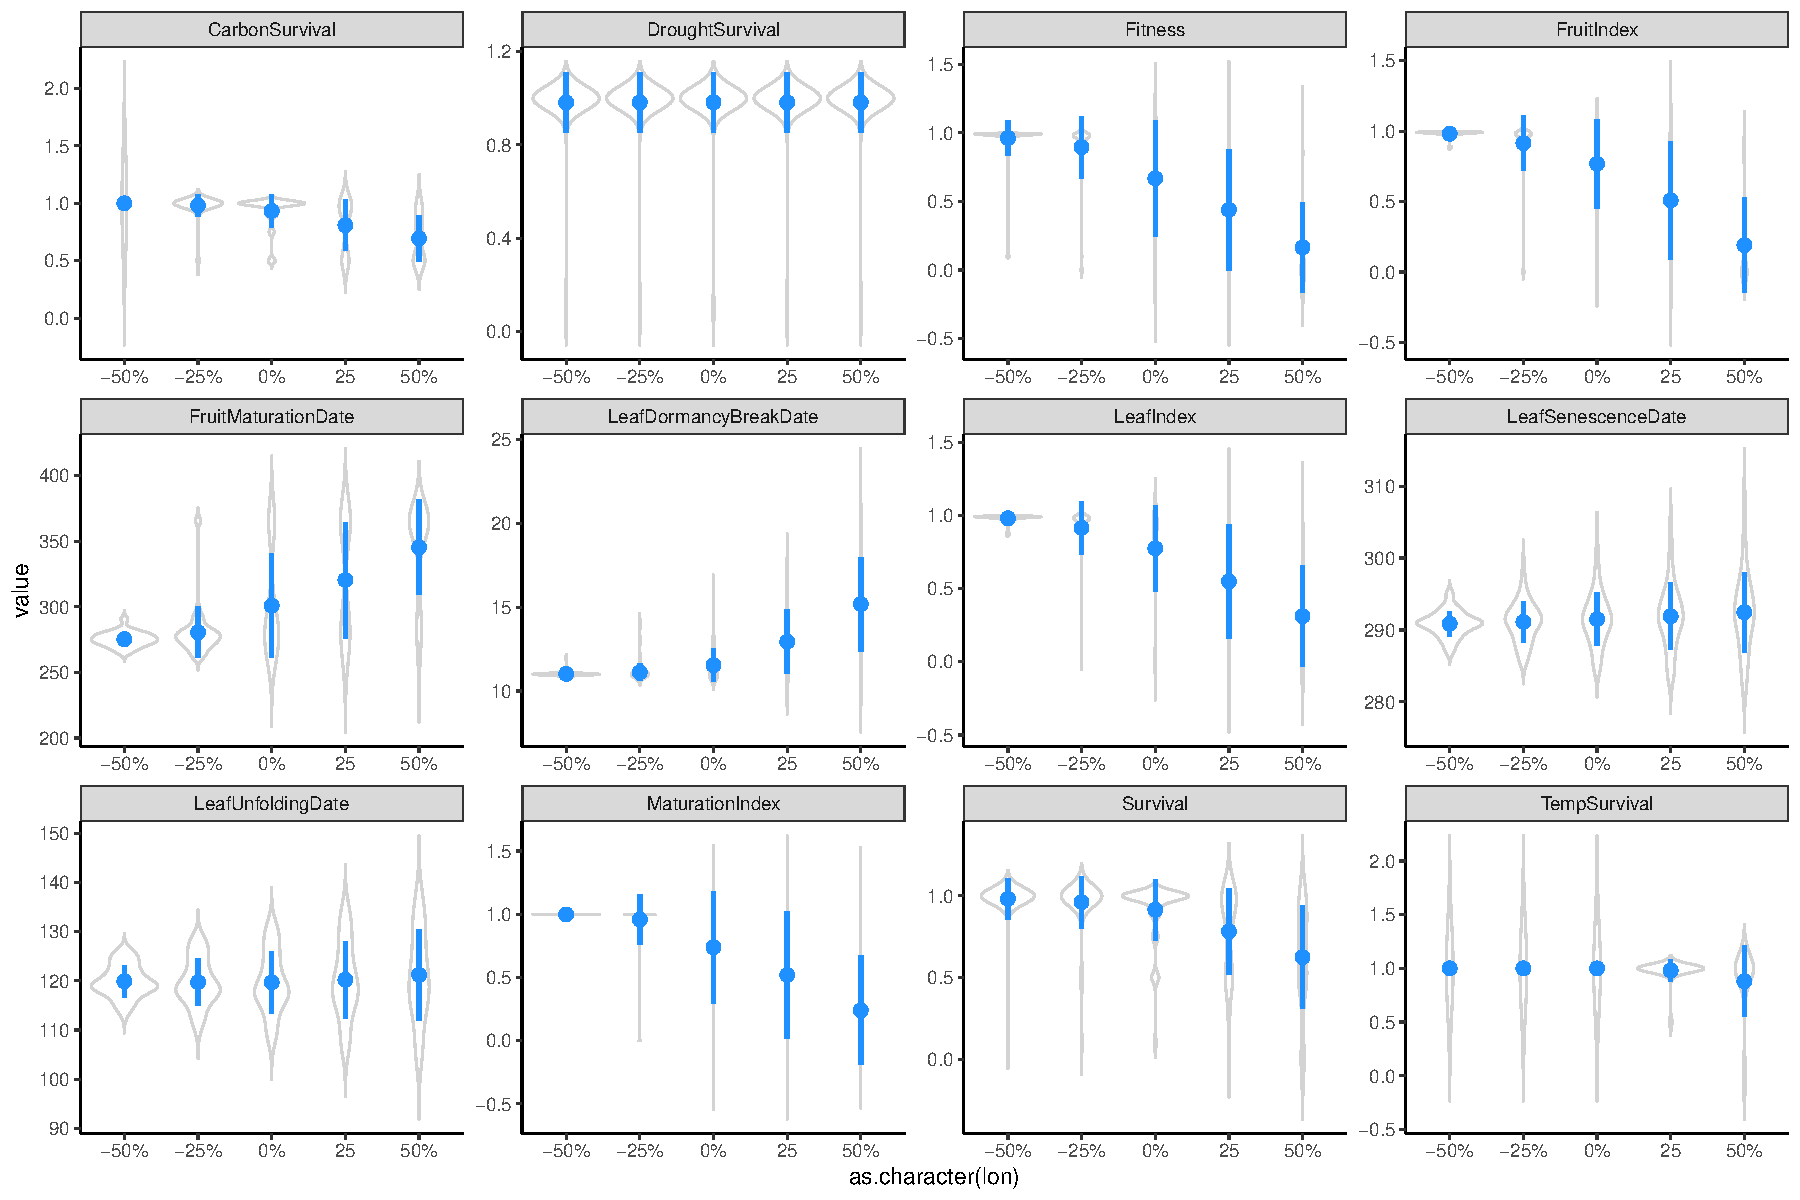
\includegraphics[width=1\textwidth]{..//analyses/graphs/phenofit/sims/sdsim53_allmetricsFS.pdf}
  \caption{\emph{Fagus} across changing variance across fitness components at 53\degree N latitude. Here's warming reduces frost and thus fruitindex goes up and survival goes up. Note that the leafdormancybreakdate also gets a little later but leafunfolding does not because the warming is still enough for get earlier leafout (and there is a buffer where early dormancybreakdate does not matter because it's too cold leaf unfolding to start. }
  \label{fig:fagussd53}
  \end{center}
\end{figure}

\clearpage

\begin{figure} 
 \begin{center}
\noindent 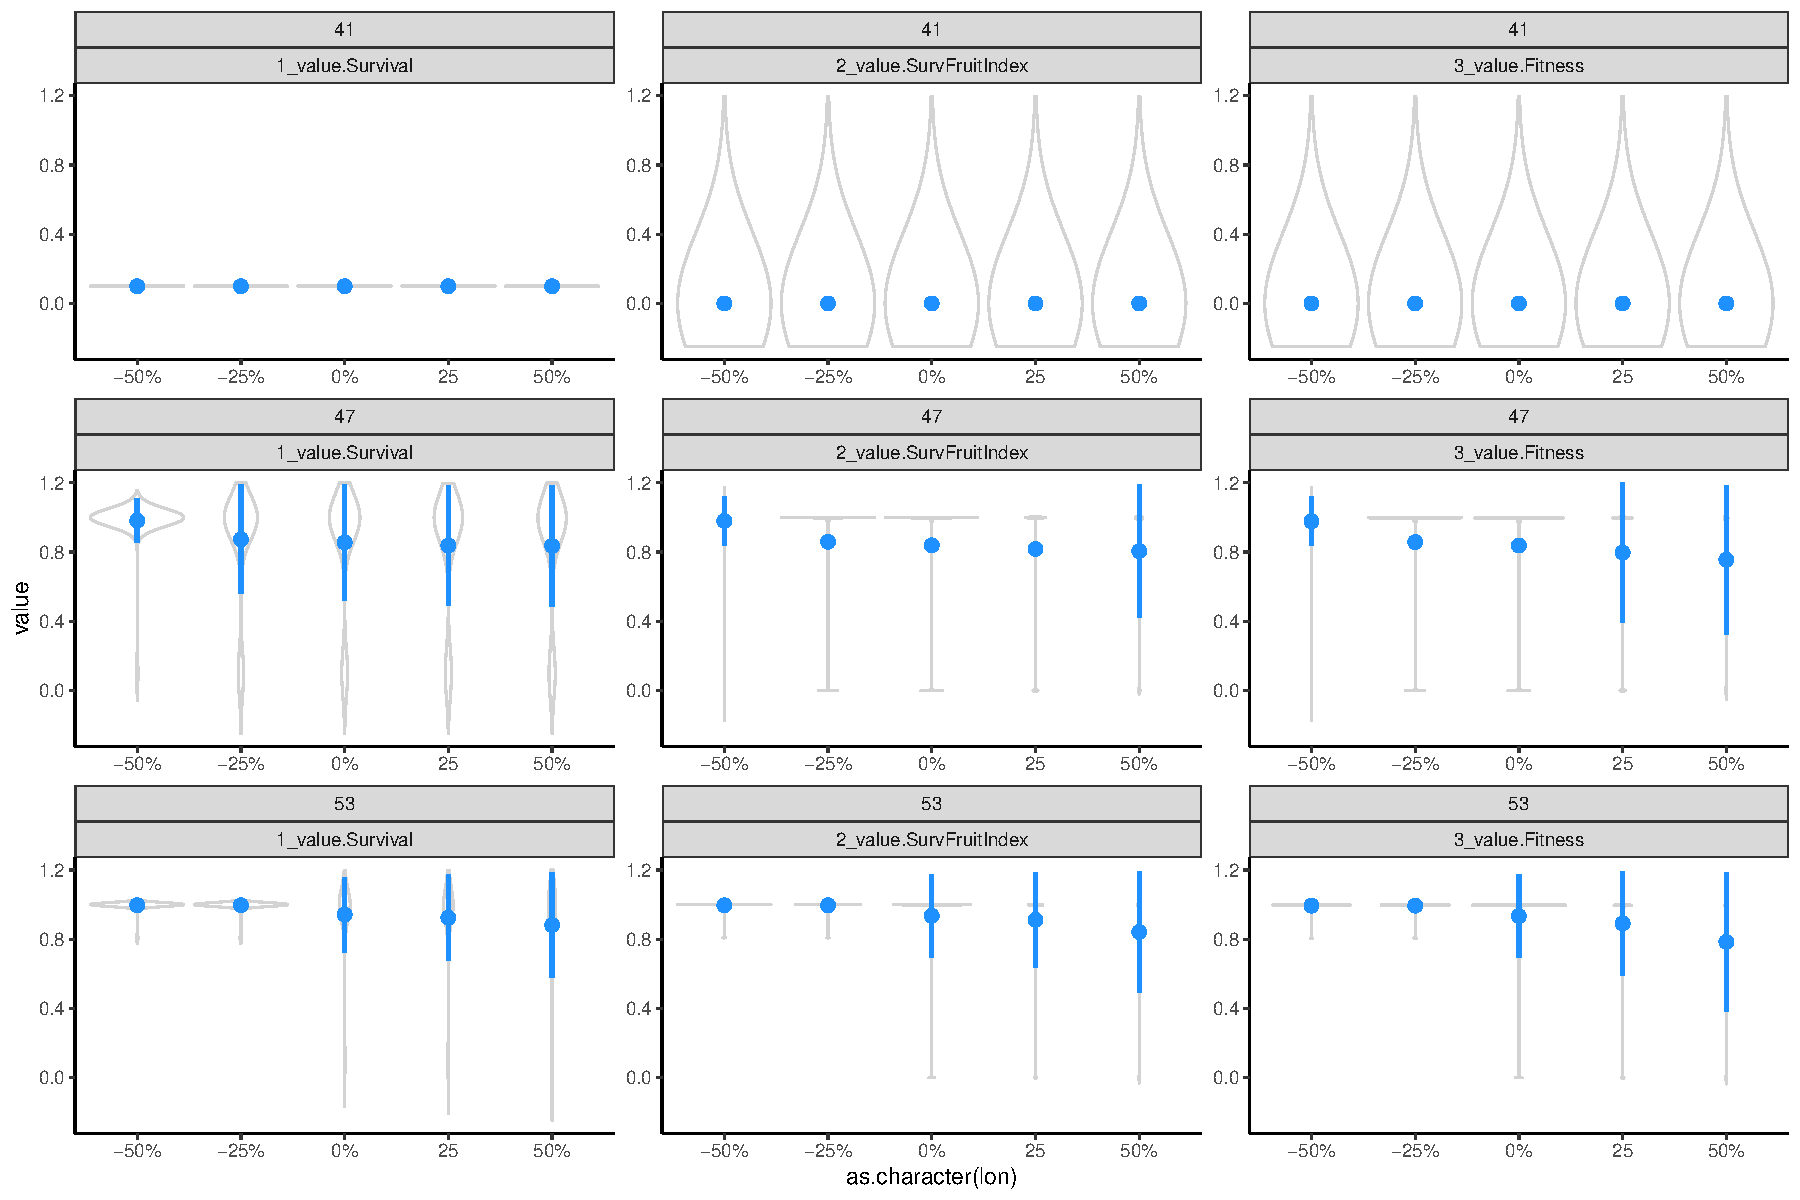
\includegraphics[width=1\textwidth]{..//analyses/graphs/phenofit/sims/metrics3/sdsim_3metricsPS.pdf}
  \caption{\emph{Pinus} across changing variance showing three latitudes. There is no survival at low latitudes, while at higher latitudes (see Fig. \ref{fig:pinussd53}) there is.}
  \label{fig:pinussd3}
  \end{center}
\end{figure}

\begin{figure} 
 \begin{center}
\noindent 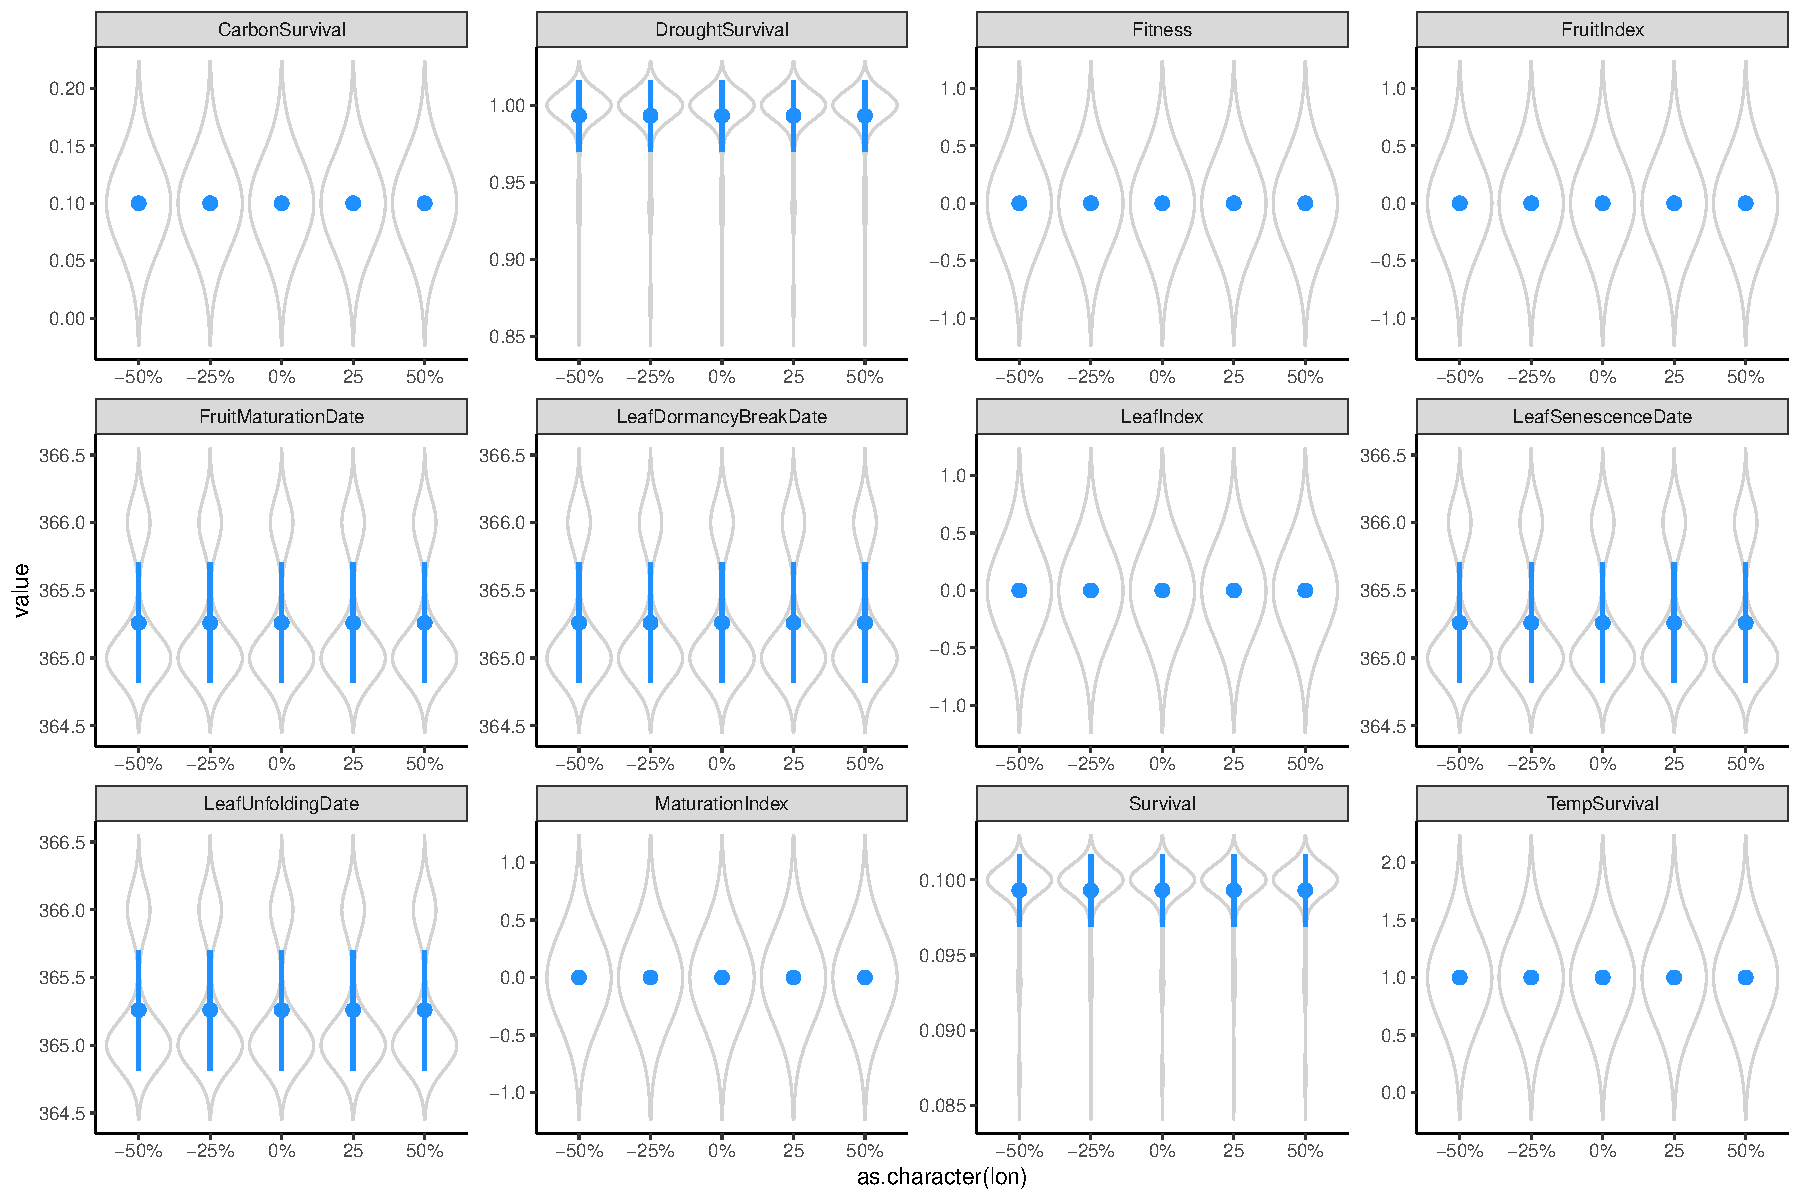
\includegraphics[width=1\textwidth]{..//analyses/graphs/phenofit/sims/sdsim41_allmetricsPS.pdf}
  \caption{\emph{Pinus} across changing variance across fitness components at 41\degree N latitude.}
  \label{fig:pinussd41}
  \end{center}
\end{figure}

\begin{figure} 
 \begin{center}
\noindent 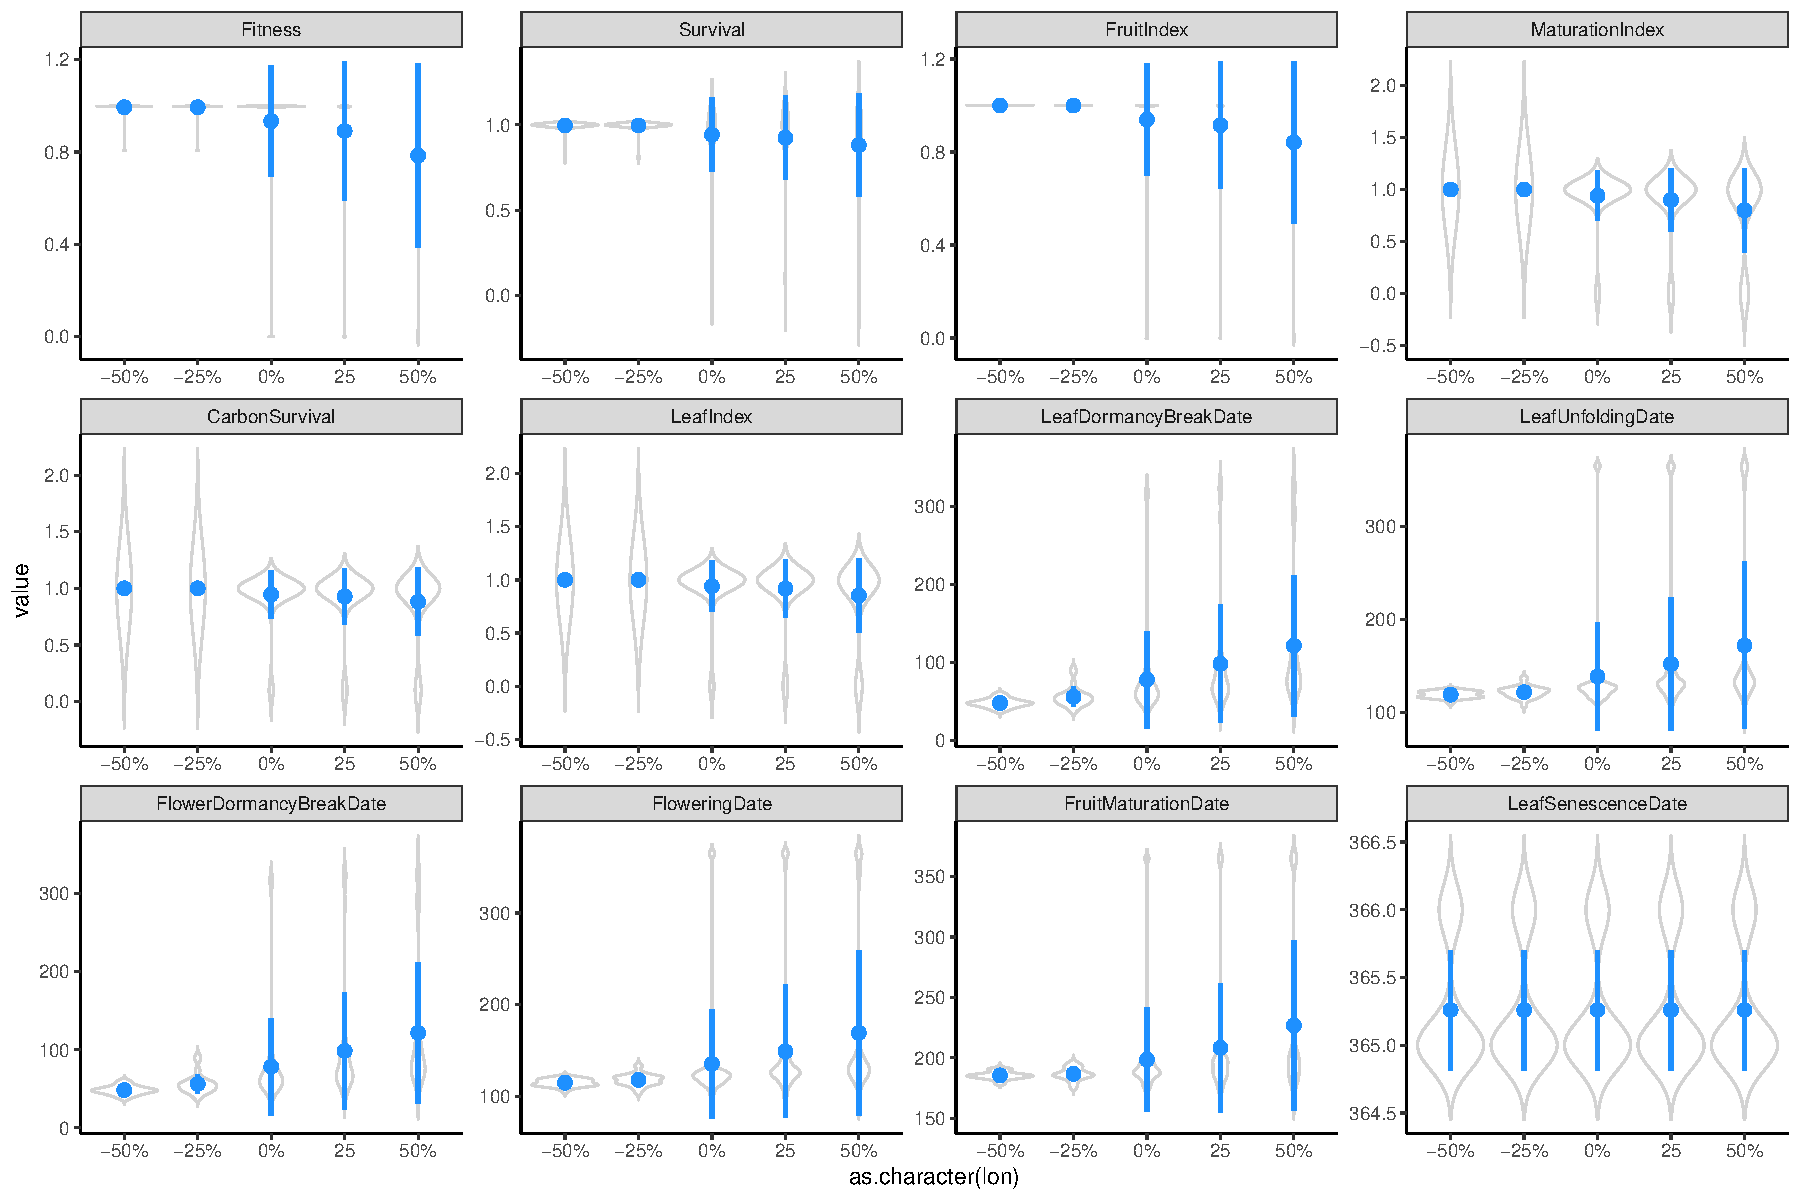
\includegraphics[width=1\textwidth]{..//analyses/graphs/phenofit/sims/sdsim53_allmetricsPS.pdf}
  \caption{\emph{Pinus} across changing variance across fitness components at 53\degree N latitude. }
  \label{fig:pinussd53}
  \end{center}
\end{figure}

\clearpage

For the sd results for \emph{Quercus} ....

\begin{figure} 
 \begin{center}
\noindent 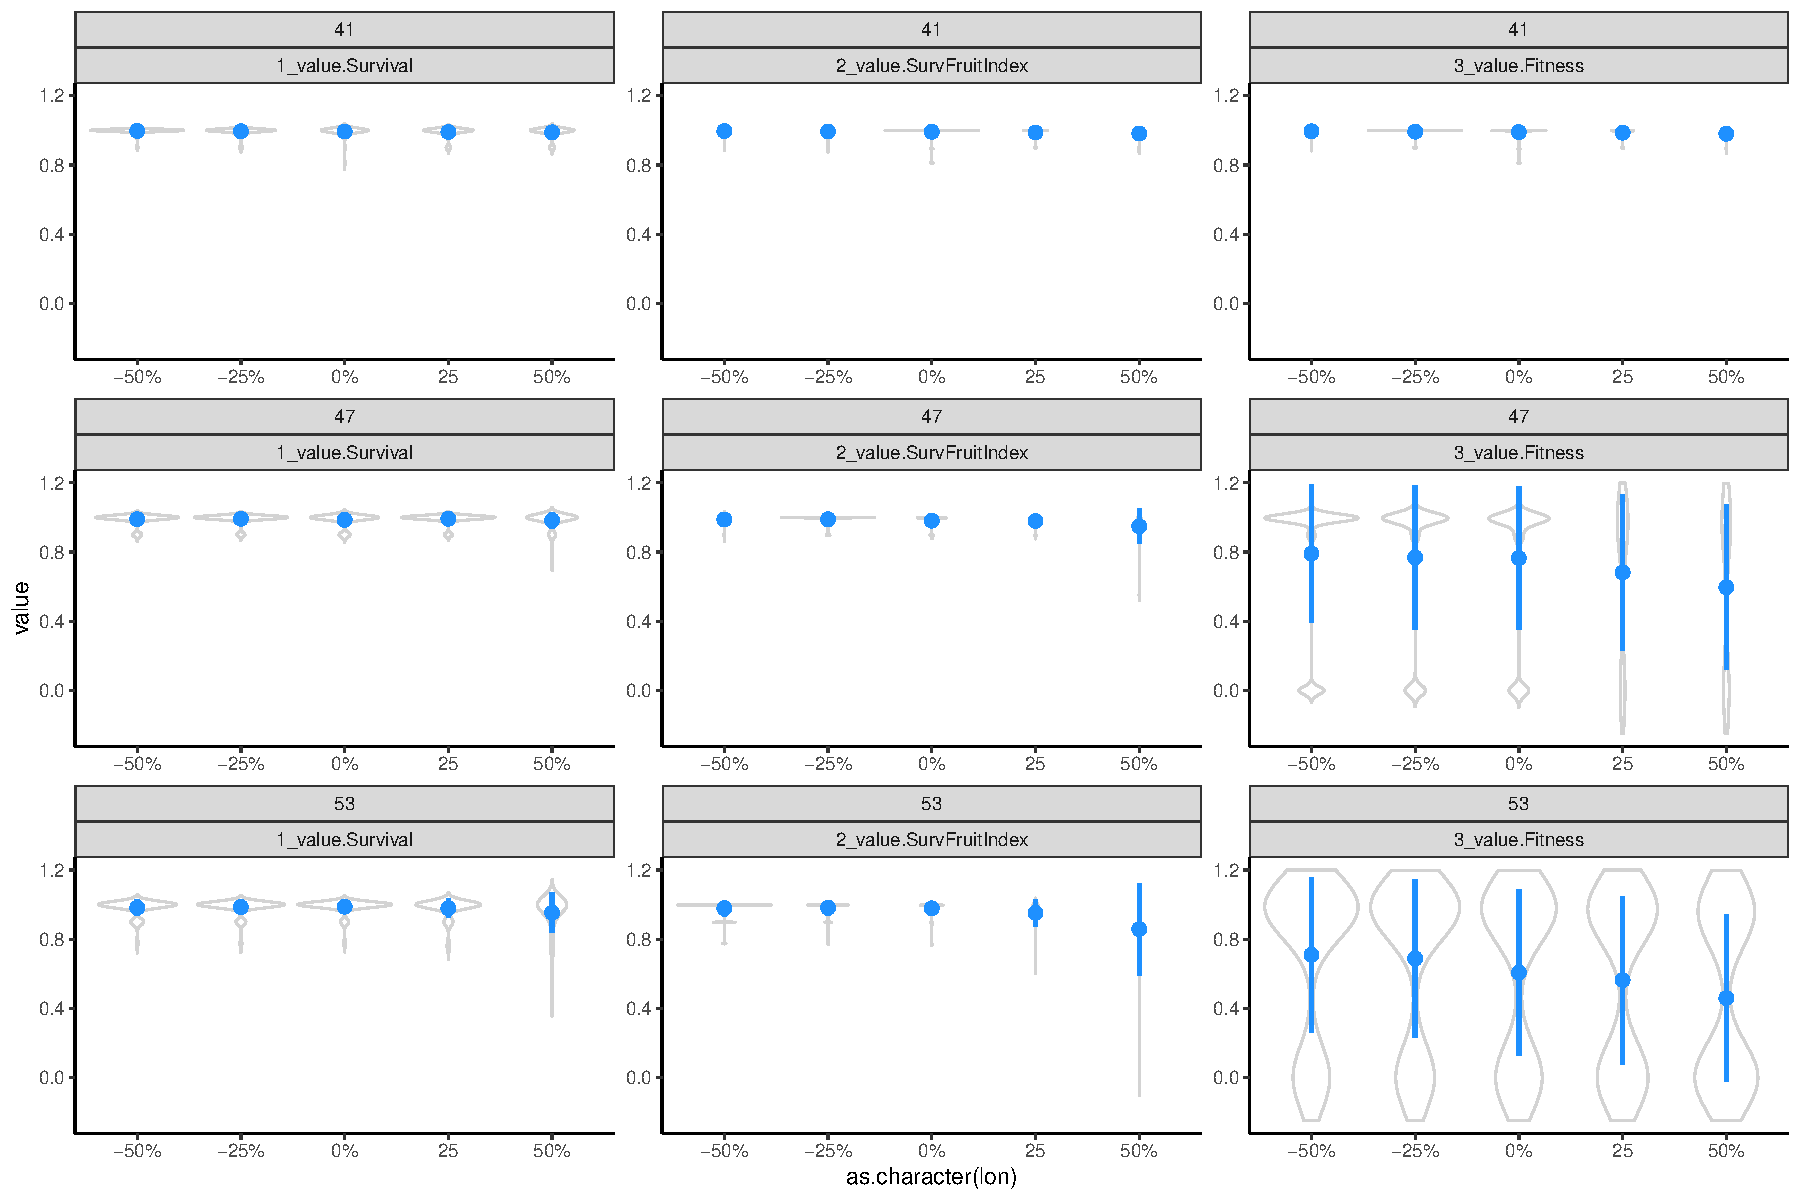
\includegraphics[width=1\textwidth]{..//analyses/graphs/phenofit/sims/metrics3/sdsim_3metricsQR.pdf}
  \caption{\emph{Quercus} across changing variance showing three latitudes.}
  \label{fig:quercussd3}
  \end{center}
\end{figure}

\begin{figure} 
 \begin{center}
\noindent 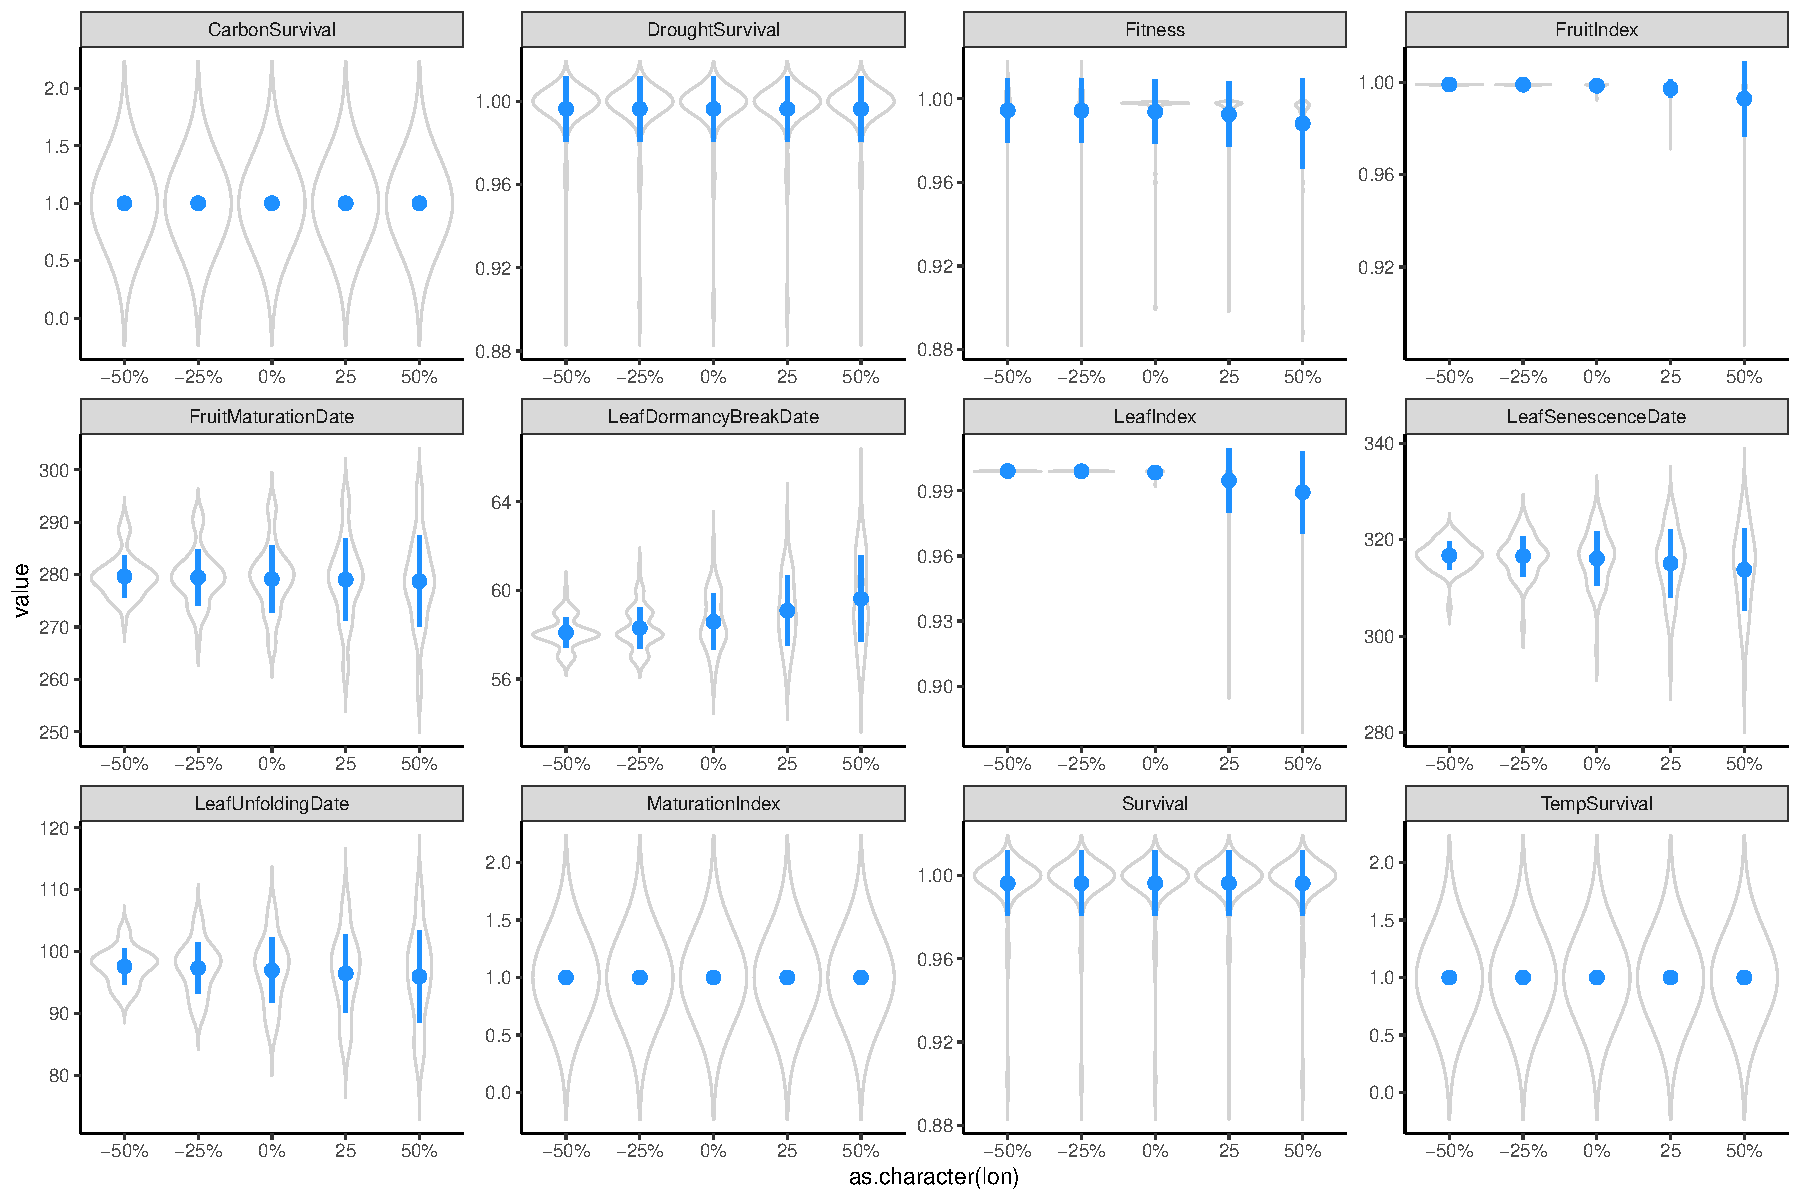
\includegraphics[width=1\textwidth]{..//analyses/graphs/phenofit/sims/sdsim41_allmetricsQR.pdf}
  \caption{\emph{Quercus} across changing variance across fitness components at 41\degree N latitude. Extremely tiny declines in fitness with increasing variance come from some frost (lower leafindex).}
  \label{fig:quercussd41}
  \end{center}
\end{figure}

\begin{figure} 
 \begin{center}
\noindent 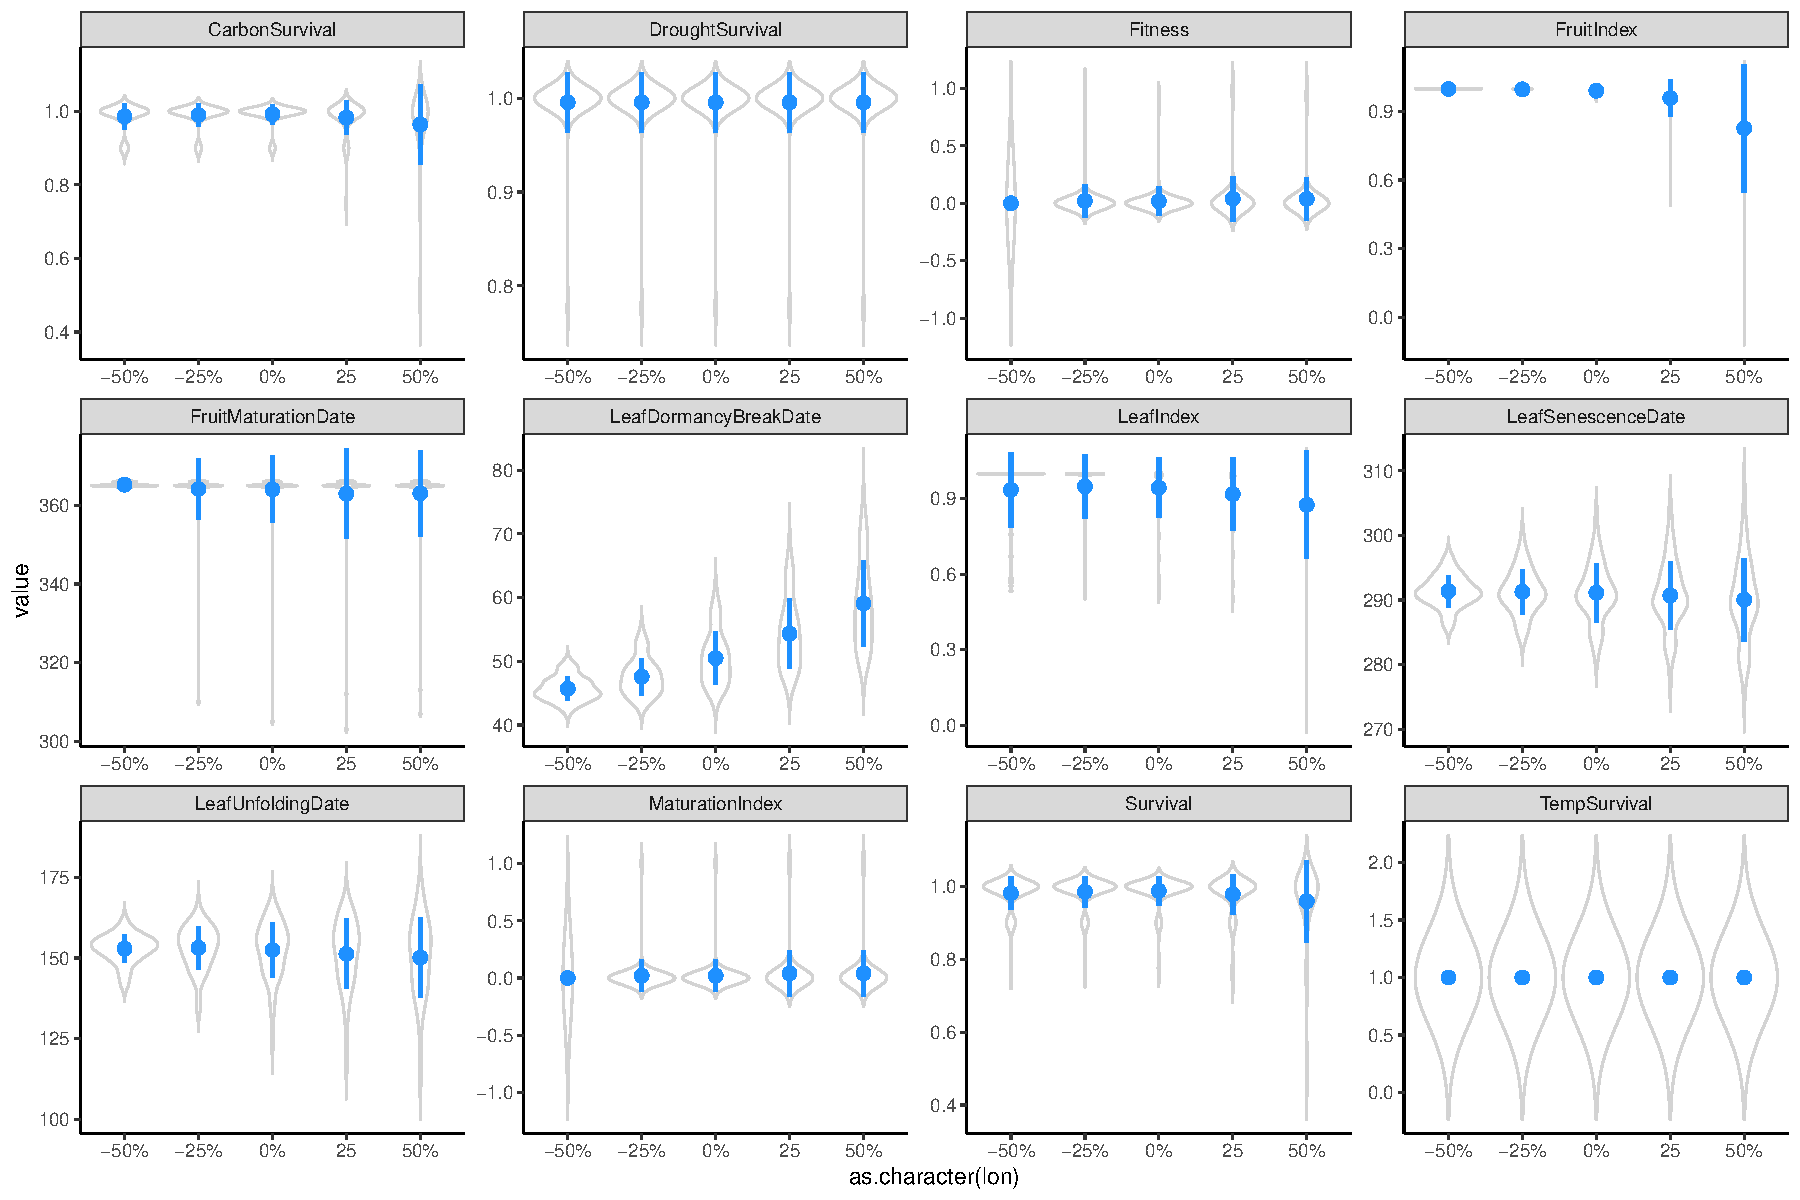
\includegraphics[width=1\textwidth]{..//analyses/graphs/phenofit/sims/sdsim53_allmetricsQR.pdf}
  \caption{\emph{Quercus} across changing variance across fitness components at 53\degree N latitude. Small declines in fitness with higher variance come from some frost (lower leafindex)}
  \label{fig:quercussd53}
  \end{center}
\end{figure}
\newpage
\section{Predictions!}

Victor and Lizzie made predictions for what we will see in simulations of increased warming crossed with -0.5 and $+0.5$ increases in variance. Lizzie added the take-home message that goes with each genus \emph{after} the meeting (we did not expect it to work out to sound so interesting---it just did). 

\begin{itemize}
\item Quercus: some positive and negative effects of more variance depending on whether warming is high or low
\begin{itemize}
\item No effects of increased variance at all of higher warming because no more frost damage, but ...
\item At lower levels of warming and increased variance may start to see lower survival due to frost damage. 
\item However, we may see that later dormancy date break actually becomes a problem % I assume we meant at higher warming and higher variance, but we did not say. 
\end{itemize}
\item Pinus: Variance and warming compound to lead to greater negative effects. 
\begin{itemize}
\item More variance and more warming will lead to even greater issues with dormancy break dates and thus lower carbon survival. 
\item Less variance will not change the negative results of increased warming, and might even make it worse as possibly the surve moves out of getting much chill at all. 
\end{itemize}
\item Fagus: Results depend on latitude, but include variance and warming compounding to greater positive effects. 
\begin{itemize}
\item Site 41 N: Increase variance could reduce negative effects of late dormancy somewhat, also less frost with increased warming x increased variance so high warming and high variance could lead to positive effects (more positive than either change alone)
\item Site 53 N: increased variance problems go away when combined with increased warming (easy to reach dormancy accumulation)
\end{itemize}
\end{itemize}

\newpage
\section{Some reminders for Lizzie... }
\begin{itemize}
\item Minimum carbon survival is 0.1. 
\item Pinus can sustain VERY low temperatures and is unlikely to have frost damage
\end{itemize}



\end{document}

